\chapter[Cosmological Solutions of \titleN$=2$ Supergravity]{Cosmological Solutions to $\N=2$ Supergravity}
\label{ch:planarstu}

This chapter contains work first published in \cite{Gutowski:2019iyo}. The original aim of this paper was to continue the previous work \cite{Dempster:2015, Mohaupt:2011aa, Errington:2014bta, Dempster:2016} on the construction of non-extremal, stationary solutions in theories of four-dimensional ${\cal N}=2$ vector multiplets coupled to gauged and ungauged supergravity, and to make contact in the extremal limit with the classification of supersymmetric near-horizon geometries. It was this original research idea that developed into the study of planar symmetric, cosmological solutions, that  then became the basis of this thesis. 

At a technical level, the work of \cite{Gutowski:2019iyo} was to extend the work of \cite{Dempster:2015} by allowing the solutions to have multiple charges. In the original work, the solutions were derived from U(1) gauged $\N = 2$ supergravity supported by a single electric charge. Solutions were found using the same method we will apply, in which the real formulation of special geometry was used to obtain analytic solutions after the reduction over the timelike coordinate. The solutions were derived using a static, planar symmetric ansatz and were called `Nernst branes' as they obeyed the strict third law of black hole mechanics: in the extremal limit, the area (density) of the black hole vanished. It was found that the solutions interpolated between two different hyperscale violating Lifshitz geometries between the horizon and the asymptotic limit. In the extremal limit, the Nernst solutions reduced to the solutions of \cite{Barisch:2011ui, Cardoso:2015wcf}. The solutions had singular behaviour: approaching the horizon, an observer would experience infinite tidal forces and in the asymptotic limit, it was found that the physical scalar fields diverge. In a second paper \cite{Dempster:2016}, the Nernst solution was realised as a boosted AdS \sch black brane in five dimensions and the divergence of the singularities when taking the asymptotic limit was resolved.

In our research \cite{Gutowski:2019iyo}, we showed that it was possible to solve the equations of motion using the same machinery of \cite{Dempster:2015} for solutions supported by two, three or four charges under Abelian gauge fields. We found that when following the solution generating technique, increasing the number of charges supported by the brane required us to reduce the number of gauge parameters and restrict the form of the prepotential. For the case of four charges, all gauge parameters are required to be set to zero, and so the model we consider simplifies from gauged to ungauged supergravity. 

It was found that for the solutions with more than one charge, the strict third law no longer held. The solution with two charges was a black hole solution, which had a single Killing horizon with finite area density in the extremal limit. In the asymptotic limit, the two-charge solution was conformally flat --- in contrast to the Lifshitz geometry of the Nernst solution, which was conformally $AdS_4$. The three-charge ansatz led to solutions for a class of gauged vector multiplet theories, including the gauged STU model, while the four-charge system was a solution to the ungauged STU model. The three- and four-charge solutions had stranger behaviour in the extremal limit. It was found that when the surface gravity was taken to be zero, the area density diverged. Furthermore, as in the planar solutions of the Einstein-Maxwell theory discussed in Section \ref{sec:emcausal}, the static patch of the three- and four-charge solution interpolated between a curvature singularity and a Killing horizon. By analytical continuation through the horizon, we obtained time-dependent regions which were asymptotic to Kasner-like solutions in the infinite past and infinite future for the three-charge solution and true-Kasner asymptotically for the four-charge solution. These solutions can be understood as `inside-out' compared to the causal structures of non-extremal black hole and black brane solutions, and should be interpreted as cosmological spacetimes. 

Our family of solutions overlaps with previously found solutions of Einstein-Maxwell-Dilaton theories and truncations of supergravity theories in the literature, which in particular display the same Penrose-Carter diagram \cite{Burgess:2002vu, Burgess:2003mk, Cornalba:2003kd}. We also find that the Penrose-Carter diagram is of the form of the diagram given in Figure \ref{fig:PC} from our discussion of the planar solutions of Einstein Maxwell theory. Studying the three- and four-charge solutions, it was found that the qualitative behaviour of their causal structure was similar enough to discuss simultaneously. It is because of this that in this thesis we choose to focus only on the ungauged, four charge solutions found in \cite{Gutowski:2019iyo}, and leave a reference to the paper for further discussion of the cosmological solution of the gauged, three-charge solutions. 

The structure of this chapter is as follows. In Section \ref{sec:stusolbg} we give sufficient background to understand the already established work of \cite{Mohaupt:2011aa, Errington:2014bta, Dempster:2015, Dempster:2016} and relate this back to our discussion from Section \ref{sec:supergravitylag} and Section \ref{sec:cmap}. In Section \ref{sec:stueucinstanton}, the three-dimensional equations of motion are solved, producing a Euclidean instanton solution. In Section \ref{sec:4dSolutions} this is uplifted to produce a four-dimensional solution, where regularity of the Killing horizon is imposed, allowing us to reduce the number of free integration constants. In Section \ref{sec:stucausal}, the four-dimensional solution is carefully considered, and we find a qualitative similarity in structure when compared to the planar symmetric solutions of the Einstein-Maxwell theory. In Section \ref{sec:emfromstu}, we will show that by taking the special limit in which all scalar fields of the solution are constant, the four-charge solution reduces to the planar symmetric solutions to Einstein-Maxwell theory.

\section{Background}
\label{sec:stusolbg}

In this section, we overview the approach developed in \cite{Mohaupt:2011aa, Errington:2014bta, Dempster:2015, Dempster:2016} to construct non-extremal, stationary solutions of $\N=2$, $D=4$ supergravity coupled to $n_V$ vector multiplets. During this chapter, we will use the following tools to obtain our static, planar symmetric, four-dimensional solutions:
\begin{enumerate}[(i)]
\item
The dimensional reduction over time to obtain an effective three-dimensional Euclidean theory.
\item
The real, rather than the more commonly used complex formulation of the special geometry of $\N=2$ vector multiplets, which is based on a Hesse potential rather than a prepotential.
\item
A set of conditions which decouples the field equations and allows us to integrate them elementarily; this requires us to impose restrictions on the admissible prepotential/Hesse potential, and to consistently truncate the field content to a subset of `purely imaginary' (PI) configurations.
\end{enumerate}
Our initial work which led to the results of this thesis began with only small modifications from previous research papers, in particular \cite{Dempster:2015}, where planar symmetry was also considered. In this section, we summarise the essential points of each of these steps to a level in which our research was carried out. For further, more technical details, we refer \cite{Mohaupt:2011aa} for a discussion of the dimensional reduction beyond what has been covered in Section \ref{sec:cmap} and \cite{Errington:2014bta, Dempster:2015, Gutowski:2019iyo} for more details on the generation of solutions of $\N =2$ (un)gauged supergravity extending to models more generic than the STU model we consider in this chapter.

Our starting point is the bosonic content of the general two-derivative Lagrangian for $n_V$ vector multiplets coupled to $\N=2$ Poincar\'e supergravity introduced in Section \ref{sec:supergravitylag}. The Lagrangian is given by 
\begin{equation}
\label{eq:4dlag}
\begin{aligned}
     \mathbf{e}_4^{-1} \La &= - \frac{1}{2}R_4 - g_{I\bar{J}} \partial_\mu X^I \partial^\mu \bar{X}^{\bar{J}} + \frac{1}{4} \I_{IJ} F^I_{\mu \nu} F^{J|\mu \nu} + \frac{1}{4} \cR_{IJ} F^I_{\mu \nu} \tilde{F}^{J|\mu \nu},
\end{aligned}
\end{equation}
where $\mu \in \{0,1,2,3 \}$ are the spacetime indices, $\mathbf{e}_4$ is the vierbein, $R_4$ is the Ricci scalar, $F_{\mu \nu}^I $ are the Abelian field strengths, $I,J \in \{ 0,1,\ldots, n_V \}$. In our conventions the tilde represents the Hodge-dual
\begin{equation}
\tilde{F}_{\mu \nu} = \frac{1}{2} \tensor{\varepsilon}{_{\mu \nu \rho \sigma}} F^{\rho \sigma} \;.
\end{equation}

As discussed in Section \ref{sec:supergravitylag}, all data in the Lagrangian is encoded by a {\em prepotential} $F=F(X^I)$, which is a holomorphic function, homogeneous of degree two in the complex scalar fields $X^I$. By working with the scalar fields of the superconformal theory, we're able to package together $(X^I, F_I)^T$, which is a symplectic vector where $F_I = \partial_I F(X^I)$. We must remember that by working with $X^I$, we introduce redundant degrees of freedom and must impose the D-gauge and fix the U(1) symmetry to work with the independent degrees of freedom of the Poincar\'e supergravity theory. The physical scalars of the Poincar\'e theory are found from ratios of the superconformal scalars 
\begin{equation}
\label{eq:physicalscalarshere}
 z^A = \frac{X^A}{X^0}, \quad \bar{z}^A = \frac{\bar{X}^A}{\bar{X}^0}, \qquad A \in \{ 1, \ldots, n_V \}.
\end{equation}
Working with the scalars $X^I$ has the advantage of formally balancing the number of scalar and vector fields. As a reminder: in Section \ref{sec:supergravitylag}, we discussed the derivation of Poincar\'e supergravity by gauge fixing the superconformal theory and that to construct the supergravity multiplet, we needed to include an additional vector multiplet to recover the graviphoton in the supergravity multiplet. 

As introduced in Section \ref{sec:electromagneticduality}, the most important feature of ${\cal N}=2$ vector multiplets is that the field equations (though not the Lagrangian) are invariant under the action of the symplectic group $\text{Sp}(2n_V+2, \mathbb{R})$, which acts linearly on the field strengths $(F^{I}_{\mu \nu}, G_{I|\mu \nu})^T$. The symplectic transformations generalise the electric-magnetic duality of the source-free Maxwell equations, and contain stringy symmetries, such as T-duality and S-duality, if the theory under consideration arises as a low-energy effective theory from string theory. By supersymmetry, the full set of field equations is symplectically invariant, with the scalars described by the symplectic vectors $(X^I, F_I)^T$.

Preserving manifest symplectic covariance is vital in our solution generating method, in that it allows a simplification of the equations of motion such that they are solved exactly. However, there is a drawback to working with the complex scalar fields $X^I$ as they do not form a symplectic vector by themselves. Similarly, the couplings $g_{I\bar{J}}$, $\I_{IJ}$ and $\cR_{IJ}$ do not transform as tensors under the symplectic group, but have a more complicated behaviour. To resolve these transformation issues, we instead work with the special real formulation, with real scalar fields $q^a$, $a \in \{1, \ldots, 2n_V+2\}$, related to the complex scalars $X^I$ by
\[
 (q^a) = \left( \begin{array}{c}
          x^I \\ y_J \\
          \end{array} \right) = \mbox{Re}
         \left( \begin{array}{c}
             X^I \\ F_I \\
            \end{array} \right) .
\]
These real scalar fields have the benefit of transforming as a vector under symplectic transformations. In this formulation, all couplings are encoded in a real function $H=H(q^a)$, called the Hesse potential, which is homogeneous of degree two, and which up to a factor, is the Legendre transform of the imaginary part of the prepotential $F$ (see \cite{Mohaupt:2011aa} for further details). It is helpful to think of the complex and real formulations of special geometry as being related to one another in the same way as the Lagrangian and Hamiltonian formulations of mechanics, see for example \cite{Cardoso:2012nh} and \cite{LopesCardoso:2019mlj} for a detailed, comprehensive discussion. 

\subsection{Dimensional reduction}
\label{sec:dimred}

As summarised above, we generate four-dimensional solutions through finding Euclidean instanton solutions in three dimensions, which we then uplift back into four dimensions. We accomplish this via a Kaluza-Klein reduction over a timelike coordinate, following the formulae given in Section \ref{sec:dimredcalc}. The general discussion of this reduction was given in Section \ref{sec:cmap}. We begin choosing a Kaluza-Klein ansatz for our four-dimensional spacetime. Following \cite{Dempster:2014}, we choose to additionally impose that our four-dimensional solutions are static, and therefore decompose the four-dimensional spacetime metric as
\begin{equation}
\label{eq:4d3d}
 ds_4^2 = - e^{\phi} dt^2 + e^{-\phi} ds_3^2 \; ,
\end{equation}
where $\phi$ and all matter fields are assumed to be independent of time $t$. The field $\phi$ is the Kaluza-Klein scalar and there is no Kaluza-Klein vector since the assumption that field configuration is static\footnote{As a reminder, staticity assumes that the metric is both stationary (time-independent) and hypersurface-orthogonal (no time-space cross-terms)} sets $V_\mu = 0$. As discussed in Section \ref{sec:supergravitylag}, by performing a field redefinition of the complex scalar fields, the Kaluza-Klein scalar $\phi$ is absorbed
\begin{equation}
\label{YX}
Y^I := e^{\phi/2} X^I \;.
\end{equation}
We do not introduce a new symbol for the corresponding real scalars $q^a$, which, are subject to the same rescaling, such that from now on we understand the real scalars are written as
\[
 (q^a) = \left( \begin{array}{c}
          x^I \\ y_J \\
          \end{array} \right) = \mbox{Re}
         \left( \begin{array}{c}
             Y^I \\ F_I(Y) \\
            \end{array} \right) \;.
\]
The advantage of this field redefinition is that the Kaluza-Klein scalar is now on the same footing as the four-dimensional scalar fields. When needed, the Kaluza-Klein scalar can be extracted as $e^\phi = - 2 H$, where $H$ is the Hesse potential considered as a function of the rescaled real scalars $q^a$. Upon dimensional reduction, the $(n_V+1)$ four-dimensional vector fields split into scalars $\zeta^I$ and three-dimensional vector fields which can be dualised into a second set of scalars $\tilde{\zeta}_I$. These $2n_V+2$ scalars can be combined into the symplectic vector $\hat{q}^a = \frac{1}{2} (\zeta^I, \tilde{\zeta}_I)^T$. We refrain from giving the explicit relations between the various fields, and refer the interested reader to \cite{Mohaupt:2011aa, Errington:2014bta, Dempster:2015}. What matters is that all dynamical degrees of freedom are now encoded in the $(4n_V+4)$ real scalars $q^a, \hat{q}^a$, which form two symplectic vectors and the four-dimensional fields can be recovered with known formula from the literature.

Following the reduction outlined in Section \ref{sec:cmap}, the resulting three-dimensional Lagrangian is given by \eq{3dlag}, repeated here for convenience 
\begin{equation*}
\begin{aligned}
 \mathbf{e}_3^{-1} \La_3 &= -\frac{1}{2}R_3 - \tilde{H}_{ab}\big(\partial_\mu q^a\partial^\mu q^b -  \partial_\mu \hat{q}^a \partial^\mu \hat{q}^b \big) \\
 &- \frac{1}{H^2} \big(q^a\Omega_{ab}\partial_\mu q^b \big)^2 +  \frac{2}{H^2}\big(q^a\Omega_{ab}\partial_\mu \hat{q}^b \big)^2. \\
\end{aligned}
\end{equation*}
where $H$ is the Hesse potential and
\[
 \Omega_{ab} = \left( \begin{array}{cc}
            0 & \mathbbm{1} \\
            - \mathbbm{1} & 0 \\
           \end{array} \right) ,
 \]
are the components of the symplectic form $\Omega = \half \Omega_{ab} dq^a \wedge dq^b$.
 
Note that in the above equation, the final line from \eq{3dlag} is missing, which is a result of the static assumption removing the Kaluza-Klein vector. The equations of motion for the Lagrangian \eq{3dlag} are derived in \cite{Mohaupt:2011aa}, but are not included here as the resulting simplification made after the following discussion will allow a more concise derivation of the equations of motion we will consider.

\subsection{Restricted field configurations}
\label{sec:restricted}
In order to obtain solutions of the field equations by decoupling and elementary integration, we make two further assumptions.

\begin{enumerate}[(i)]
\item We will need to know the Hesse potential explicitly, but models are naturally defined in terms of their prepotential, \textit{e.g.} in the context of Calabi-Yau compactifications of string theory. Since the Hesse potential is obtained by a Legendre transformation of the (imaginary part of the) prepotential, it cannot be computed in closed form for a generic prepotential. We will therefore restrict the form of the prepotential in such a way that we can obtain the Hesse potential explicitly. 
\item We want the field equations to decouple. This is achieved by imposing a block structure, where the scalar fields within each block are proportional to each other, and where equations within a block do not couple to equations in other blocks. Such block structures appear if we consistently truncate out part of the scalar fields.
\end{enumerate}
We remark that the two types of conditions we impose are not independent. We only need to know a Hesse potential for the subset of fields which are not truncated out consistently. The more fields we truncate out, the larger the class of prepotentials admissible. In \cite{Gutowski:2019iyo}, as we increased the number of charges, the fields kept in the effective three-dimensional theory became more and more restricted. In \cite{Dempster:2015}, it was shown that this restriction must also be applied to the gauging parameters of the scalar potential and that this required factorisation of the admissible prepotentials. In this thesis, we look at the extreme limit of this, in which we allowed the maximal number of distinct charges using this method, and in doing so, set all gauging parameters to zero, fixing the form of the prepotential by requiring it was fully factored.

For the single-charged Nernst brane solutions \cite{Dempster:2015} of gauged supergravity, it is sufficient to restrict the prepotential to be of the so-called very special form
\begin{equation}
\label{eq:veryspecial}
F(Y) = \frac{f(X^1,\ldots X^n)}{X^0} ,
\end{equation}
where $f$ is a homogeneous polynomial of degree three. This condition is equivalent to imposing that the vector multiplet theory can be lifted to five dimensions. In \cite{Gutowski:2019iyo}, we found that increasing the number of charges required factorising the polynomial $f(X^1,\ldots X^n)$ such that the prepotentials were of the form
\begin{equation}
\label{prepotentials}
\begin{aligned}
    F_2(X) = \frac{X^1 f_2(X^i,\ldots,X^n)}{X^0}\;,
    & \quad F_3(X) = \frac{X^1 X^2 f_3(X^i,\ldots,X^n)}{X^0}\;,
     \\ F_4(X) &= \frac{X^1 X^2 X^3}{X^0} \;,
\end{aligned}
\end{equation}
where the subscripts count the number of charges present in the theory, and $f_2$ and $f_3$ are homogenous polynomial of degree two and one respectively. While $F_2(X)$ is still the generic form for a compactification of the heterotic string on $K3 \times T^2$ at string tree level, $F_4(X)$ is the well known STU model \cite{Duff:1995sm}, which is also the minimal example for a prepotential of the form $F_3(X)$. While more general models can be defined and solved for by relaxing the condition that $f_3$ is a polynomial, we do not know how such models could be embedded into string theory and so restricted ourselves to the polynomial case. We have included this discussion of the lower charge solutions as an illustration of how we came to the STU model for the four charge case, but we will not further discuss the form their solutions, which are explained in full detail in \cite{Gutowski:2019iyo}.

Next we specify the consistent truncation of the scalar fields $q^a,\hat{q}^a$ that we impose to achieve decoupling. In \cite{Errington:2014bta}, the truncated field configurations were called `purely imaginary' (PI) because the corresponding four-dimensional physical scalars $z^A$ are purely imaginary, and in terms of real scalar fields, the PI conditions require that
\begin{equation*}
	y_0 = u^0 = 0, \qquad x^A = 0, \qquad A \in \{1,\ldots, n_V\}.
\end{equation*}
This type of condition is also known as `axion-free', as in our parametrisation, the real parts of $z^A$ have an axion-like shift symmetry for prepotentials of the very special form. Remembering back to the gauge fixing conditions we must impose on the complex scalars $X^I$, we can identify one of these conditions not as a restriction on the physical scalars, but instead as the condition to fix the U(1) gauge symmetry. Any of these conditions is appropriate for this gauge fixing, but it is standard to think of Im$Y^0 = 0 \Rightarrow u^0 = 0$ to be the gauge fixing condition.
%\footnote{Underlying this is that when we when do the full stationary reduction, we have $4n_V + 5$ fields, from $q^A, \hat{q}^A$ and the dualised KK Vectors. These form a symplectic vector and a symplectic scalar, but only $4n_V +4$ of the fields are independent, because of the local U(1) symmetry. As we break the U(1) symmetry we necessarily break our symplectic symmetry and so we wait until needed to remove our redundancy.} 

In terms of three-dimensional scalars, the PI condition takes the form
\begin{equation}
\label{eq:PI1}
 (q^a) \big|_{\text{PI}} = (x^0,\ldots,0;0,y_1,y_2,\ldots,y_n).
\end{equation}
This is extended to the scalars $\hat{q}^a$ which correspond to four-dimensional gauge fields by
\begin{equation}
\label{eq:PI2}	
 (\partial_\mu \hat{q}^a) \big|_{\text{PI}} = \half (\partial_\mu \zeta^0,\ldots,0;0,\partial_\mu \zeta_1,\partial_\mu \zeta_2,\ldots,\partial_\mu \zeta_n).
\end{equation}
We remark that the PI condition maintains that the solution we obtain is a consistent truncation of the full theory. A point of view we do not deeply discuss in this thesis is realising the scalar fields as harmonic maps to a target space geometry. Understanding the scalar fields as coordinates on the target manifold, making a field restriction can be interpreted as picking out some sub-manifold from the target space. From this perspective, the PI condition as a consistent truncation reflects the existence of a distinguished totally geodesic\footnote{Here, totally geodesic means that geodesics on the subspace are geodesics in the full space.} $(2n_V +2)$-dimensional sub-manifold of the $(4n_V + 4)$-dimensional scalar manifold realised from the three-dimensional effective theory obtained from dimensional reduction. 

For notational convenience, we adjust the assignment of indices $a,b,\dots$ to the scalar fields $q^a, \hat{q}^a$ such that the non-constant scalars correspond to indices $a \in \{1, \ldots, n_V+1 \}$. We can further simplify the equations of motion through some simple manipulations. All terms in the three-dimensional Lagrangian and field equations which do not involve the scalar potential either involve the constant anti-symmetric matrix $\Omega_{ab}$ or the Hesse potential $H$ and its derivatives. Looking at \eq{PI1} and \eq{PI2}, we find that 
 \begin{equation*}
 	q^a \Omega_{ab} \partial^\mu q^b = q^a \Omega_{ab} \partial^\mu \hat{q}^b = 0 .
 \end{equation*}
 Moreover, we replace the scalar fields $q^a$ by their duals $q_a = \tilde{H}_a = -\tilde{H}_{ab} q^b$, where we used that $\tilde{H}_{ab}$ are homogeneous functions of degree $-2$. While in general we cannot lower indices on $\hat{q}^a$ in the same way,\footnote{We do not require the functions $\hat{q}_a$ to be well defined on the scalar manifold, and in particular, we cannot find coordinates by computing $\tilde{H}_{ab} \hat{q}^b$ unless $\tilde{H}_{ab}$ is itself constant. This is because the above coordinate could not be consistent with $\dot{\hat{q}}_a = \tilde{H}_{ab} \dot{\hat{q}}^b$. However, $\hat{q}^a$ are well defined functions on the scalar manifold, and from this $\dot{\hat{q}}^a$ and $\dot{\hat{q}}_a$ are well defined vector and covector fields respectively.} we can lower the indices after differentiation: $\partial_\mu \hat{q}_a := \tilde{H}_{ab} \partial_\mu \hat{q}^b$ \cite{Errington:2014bta}. As the fields $\hat{q}^a$ are essentially the four-dimensional gauge potentials, which only enter into the field equations through their derivatives, this is sufficient for rewriting all field equations with indices $a$ in the lower position. Putting this all together, under the PI condition, the effective three-dimensional Lagrangian is simply
\begin{equation}
\label{eq:effective3slag}
 \mathbf{e}_3^{-1} \La_3 = -\frac{1}{2}R_3 - \tilde{H}^{ab}\big(\partial_\mu q_a\partial^\mu q_b -  \partial_\mu \hat{q}_a \partial^\mu \hat{q}_b \big).
\end{equation}


\section{Euclidean instanton solutions}
\label{sec:stueucinstanton}
 We are now in the position to formulate the problem that we will solve. Starting from the Lagrangian \eq{4dlag}, we impose that the four-dimensional metric (\ref{eq:4d3d}) is static, the PI truncation (\ref{eq:PI1}, \ref{eq:PI2}) and finally that the three-dimensional metric has planar symmetry
	\begin{equation}
	\label{eq:3dplanaransatz}
	ds_3^2 = e^{4\psi} d\tau^2 + e^{2\psi} (dx^2 + dy^2).
	\end{equation}
	All fields, including the unknown function $\psi$, depend only on the overall transverse coordinate $\tau$ in this brane-like ansatz.

The resulting equations of motion can be derived from \eq{effective3slag}, alternatively, the restrictions discussed can be applied to the general three-dimensional equations for timelike dimensional reduction derived in \cite{Mohaupt:2011aa} by imposing our field restrictions. Either way, the resulting equations of motion are given by
\begin{equation}
\label{eq:eom1}
\nabla^2 \hat{q}_a = 0,
\end{equation}
\begin{equation}
\label{eq:eom2}
\nabla^2 q_a + \frac{1}{2}\partial_a \tilde{H}^{bc}(\partial_\mu q_b \partial^\mu q_c - \partial_\mu \hat{q}_b \partial^\mu \hat{q}_c) = 0,
\end{equation}
\begin{equation}
\label{eq:eom3}
-\frac{1}{2} R_{(3)\mu\nu} - \tilde{H}^{ab}(\partial_\mu q_a \partial_\nu q_b - \partial_\mu \hat{q}_a \partial_\nu \hat{q}_b) =0.
\end{equation}
The first line gives the equations of motion for for the scalars $\hat{q}^a$, which correspond to the four-dimensional vector field equations. The second line give the equations for the scalars $q^a$, which encode the four-dimensional scalars $z^A$ and the Kaluza-Klein scalar $\phi$. The last line are the three-dimensional Einstein equations which determines the three-dimensional warp factor $\psi$.

To solve Einstein's equations we use that the non-zero components of the Ricci tensor are found to be
\begin{equation*}
 R_{\tau \tau} = 2 \ddot{\psi} - 2\dot{\psi}^2, \quad R_{xx} = R_{yy} = e^{-2\psi} \ddot{\psi},
\end{equation*}
where we use a dot to denote differentiation by $\tau$. The equations \eq{eom3} then reduce to the following form for $\mu, \nu \neq \tau$
\begin{equation}
\label{eq:eom4}
\frac{1}{2}e^{-4\psi}\ddot{\psi} = 0 ,
\end{equation}
and for $\mu, \nu = \tau$
\begin{equation}
\label{eq:eom5}
\tilde{H}^{ab} \big(\dot{q}_a \dot{q}_b - \dot{\hat{q}}_a \dot{\hat{q}}_b \big) = \dot{\psi}^2 - \tfrac{1}{2} \ddot{\psi},
\end{equation}
where we have substituted in \eq{eom4} to reduce this condition. We remark that \eq{eom5} is called the Hamiltonian constraint \cite{Errington:2014bta,Dempster:2015}.

We are interested in deriving solutions carrying charge under four gauge fields. The requires enforcing that the equations of motion for all $q_a$ decouple, which in turn requires that the prepotential takes the form
\begin{equation}
        F(X) = \frac{X^1 X^2 X^3}{X^0},
\end{equation}
which is the well-known prepotential of the STU model. 

From the STU prepotential, we can compute the Hesse potential \eq{hessepotential}
\begin{equation}
\label{eq:stuhesse}
H = -\frac{1}{4} (-q_0 q_1 q_2 q_3)^{-\half} \;,
\end{equation}
and as we know the exact form of the Hesse potential, we can now completely solve for the metric, which is diagonal with elements given by
\begin{equation*}
  \tilde{H}^{aa} = \frac{1}{4q_a^2} \; .
\end{equation*}
We note that after making the PI restriction we have reduced from four complex to four real variables.

We start by solving the equations of motion for $\hat{q}_a$. Since all fields are assumed to only depend on $\tau$, Equation \eq{eom1} reduces to
\begin{equation}
\ddot{\hat{q}}_a = 0.
\end{equation}
Integrating up we obtain
\begin{equation}
\dot{\hat{q}}_a = K_a.
\end{equation}
The non-vanishing constants $K_a$ are proportional to the electric charge $Q_0$ and magnetic charges $P^A$ of the four gauge fields in this
solution\footnote{The minus sign in front of $Q_0$ reflects that $K_a$
transforms as a covector, and not as a vector, under symplectic transformations.}
\begin{equation}
\label{eq:eom6}
\dot{\hat{q}}_a = K_a = (-Q_0, 0, 0, 0; 0, P^1, P^2, P^3).
\end{equation}

Now turning to the scalar fields $q_a$, studying \eq{eom2} we find that they completely decouple from each other, and we obtain four differential equations
\begin{equation}
\ddot{q}_a - \frac{\dot{q}^2_a - K_a^2}{q_a} = 0.
\end{equation}
This can be integrated to obtain the form for the scalar fields
\begin{equation}
q_a = \pm \frac{K_a}{B_a} \sinh \bigg(B_a \tau + B_a \frac{h_a}{|K_a|} \bigg),
\end{equation}
where the integration constants have been collected together as
\begin{equation*}
  B_a = (B_0,B_1,B_2,B_3), \quad h_a = (h_0, h^1, h^2, h^3).
\end{equation*}
Without loss of generality we set $B_a \geq 0$. To avoid curvature singularities associated with zeros of the fields $q_a$, we further require that sign($h_0$) = sign($Q_0$) and sign($h^A$) = sign($P^A$). This ensures that there are no zeros for the domain $0 \leq \tau < \infty$.

Finally, we turn to Einstein's equations \eq{eom3}. From \eq{eom4} we have the simple result
\begin{equation*}
-\half e^{-4\psi} \ddot{\psi} = 0 \quad \Rightarrow \quad \ddot{\psi} = 0.
\end{equation*}
The Hamiltonian constraint \eq{eom5} allows us to find
\begin{equation}
\frac{1}{4q_a^2} \left(\dot{q}_a^2 - \dot{\hat{q}}_a \right) = \dot{\psi}^2 - \half \ddot{\psi} = \frac{B_0^2 + B_1^2 + B_2^2 + B_3^2}{4} \; ,
\end{equation}
Combining these results together, we can find a solution for the warp factor
\begin{equation*}
\dot{\psi} = \pm \frac{\sqrt{\sum_iB_i^2}}{2} \quad \Rightarrow \quad \psi = \pm \frac{\sqrt{\sum_iB_i^2}}{2}\tau + a_0.
\end{equation*}
As it appears in an exponential in the line element \eq{3dplanaransatz}, we additionally calculate
\begin{equation}
e^{-4\psi} = e^{-4a_0} e^{\pm 2\sqrt{\sum_iB_i^2} \tau} \; .
\end{equation}
To summarise, we have found the following planar symmetric solution to the time-reduced STU model:
\begin{equation}
    \begin{aligned}
      \dot{\hat{q}}_a &= K_a, \\
      q_a &= \pm \frac{K_a}{B_a} \sinh \bigg(B_a \tau + B_a \frac{h_a}{K_a} \bigg), \\
         e^{-4\psi} &= e^{-4a_0} e^{\pm 2\sqrt{\sum_i B_i^2} \tau} \; .\label{STU1}
    \end{aligned}
\end{equation}


\section{Four-dimensional planar solutions}
\label{sec:4dSolutions}

In this section, we study the three-dimensional instanton solutions derived as candidates for black hole solutions in four dimensions. Part of this process involves imposing regularity conditions on the matter content through placing conditions on the integration constants. 

As we mentioned in the reduction of the brane configurations in Section \ref{sec:intersecting}, to have well behaved solutions, the scalar fields must be regular on the horizon. From the point of view of $\N = 2$ supergravity coupled to vector multiplets, this condition can be traced back to ensuring certain properties of the prepotential. In our case, when the prepotential is of the very special form \eq{veryspecial}, we require that the polynomial function $f(X^1, \ldots X^n)$ have no zeros or poles. For the STU model, where $f(X) = X^1 X^2 X^3$, this translates to the simple condition that the scalars $z^A$ do not diverge on the horizon. When considering multi-charged solutions \cite{Gutowski:2019iyo}, the argument must be made for more generic prepotentials.

We can explicitly write down the four-dimensional, static, planar symmetric line element using \eq{4d3d} and \eq{3dplanaransatz}
\begin{equation}
\label{eq:ansatz}
ds_4^2 = -e^\phi dt^2 + e^{-\phi + 4\psi}d\tau^2 + e^{-\phi + 2\psi} (dx^2 + dy^2),
\end{equation}
where the Kaluza-Klein scalar is found from the Hesse potential via \eq{stuhesse}
\begin{equation*}
	e^\phi = -2H = \half \left(-q_0 q_1 q_2 q_3 \right)^{-\half}.
\end{equation*}
We can perform the lift from the three-dimensional fields into four dimensions using the dimensional reduction formulae found originally in \cite{Mohaupt:2011aa,Errington:2014bta,Dempster:2015}.

The four-dimensional physical scalars are determined by the three-dimensional scalars through the relations \cite{Errington:2014bta}
\begin{equation}
Y^0 = -\frac{1}{4q_0}, \qquad Y^A = -\frac{i}{2}e^\phi q_A,
\end{equation}
where $Y^I$ are rescaled scalar fields defined in (\ref{YX}). This yields the form for the physical scalars via \eq{physicalscalarshere}
\begin{equation}
\label{eq:gensca}
z^A = -i \bigg( -\frac{q_0 q_A^2}{q_1 q_2 q_3} \bigg)^{\half} \; .
\end{equation}
The four-dimensional gauge fields are calculated using $\hat{q}_a$ through the relation
\begin{equation}
\label{eq:gauge1}
    \hat{q}^a = \half \pvec{\zeta^I}{\tilde{\zeta}_I},
\end{equation}
where as displayed in (\ref{sec:dimred}), $\zeta^I$ are the components of the gauge fields along the reduction dimension and $\tilde{\zeta}_I$ are the Hodge duals of the three-dimensional vectors. Their relation to the four-dimensional gauge fields can be calculated from \cite{Errington:2014bta}
\begin{equation}
\label{eq:gauge2}
    \partial_\mu \zeta^I := F_{\mu t}^I, \qquad \partial_\mu \tilde{\zeta}_I := G_{I | \mu t},
\end{equation}
where we remind the reader that
\begin{equation}
\label{eq:gauge3}
    G_{I|\mu \nu} := \mathcal{R}_{IJ} F^J_{\mu \nu} - \I_{IJ} \tilde{F}^J_{\mu \nu},
\end{equation}
is the dual field strength.

We begin by looking for the location of a Killing horizon. As the solution is static, we have the timelike Killing vector field $k^\mu = \partial_t$ and we can compute its norm $k^2 = e^\phi$. Evaluating this in the limit of $\tau \rightarrow \infty$, we find that the norm of the Killing vector falls off as
\begin{equation*}
	k^2 = \exp \left(-\frac{B_0 \tau}{2} -\frac{B_1 \tau}{2} -\frac{B_2 \tau}{2} -\frac{B_3 \tau}{2} \right) \xrightarrow[\tau \rightarrow \infty]{}0 \;,
\end{equation*}
where we use that $B_i > 0$. We understand that there is a Killing horizon located in the four-dimensional spacetime for $\tau \rightarrow \infty$. We can now take the same limit for the scalar fields \eq{gensca} and ensure that they are finite on the horizon. Inserting in our result for the scalar fields $q_a$, we find the tau dependence of the physical scalars on the horizon goes as:
\begin{equation*}
  \begin{aligned}
  z^1 \big|_{\tau \rightarrow \infty} &\sim \exp \left[ \left(B_0 + B_1 - B_2  - B_3 \right)\tau \right] ,\\
   z^2 \big|_{\tau \rightarrow \infty} &\sim \exp \left[ \left(B_0 + B_2 - B_1 - B_3 \right)\tau \right] ,\\
  z^A \big|_{\tau \rightarrow \infty} &\sim \exp \left[ \left( B_0 + B_3 - B_2 - B_1 \right)\tau \right] .\\
  \end{aligned}
\end{equation*}
Imposing that these fields are finite in the limit $\tau \rightarrow \infty$ requires that the following three conditions hold:
\begin{equation*}
  \begin{aligned}
      B_0 + B_1 - B_2 - B_3 = 0 ,\\
        B_0 + B_2 - B_1 - B_3 = 0 ,\\
         B_0 + B_3 - B_2 - B_1 = 0 .
  \end{aligned}
\end{equation*}
This is satisfied when the integration constants obey $B_0 = B_1 = B_2 = B_3 = B$. The integration constant $a_0$, which appears in the warp factor, can be removed by a suitable shift in the $\tau$ coordinate and after performing the shift, we see the that the warp factor simplifies, up to a sign
\begin{equation*}
    e^{-4\psi} = e^{\pm 4 B \tau} \; .
\end{equation*}
We can set this sign through our final condition, looking at the area density of the horizon. The area of the horizon is given by integral
\begin{equation}
A = \int dx dy e^{-\phi+2\psi}\bigg|_{\tau \rightarrow \infty}.
\end{equation}
As with the planar symmetric solutions of the Einstein-Maxwell theory, our $x$ and $y$ coordinates are not compact, and so the area diverges, reflecting the planar symmetry of our ansatz. To obtain finite quantities we could identify $x,y$ periodically, but as with our discussion in Chapter \ref{ch:planarem}, we prefer to work with densities instead and take ratios relative to the coordinate area. As there are many more functions and integration constants to keep track of in this chapter, we formally set
\begin{equation*}
	\omega = \int_{\Real^2} dx \wedge dy = 1 \;,
\end{equation*}
rather than keep $\omega$ explicit in our computations. With this understood, we find that the area density of the horizon is found to be
\begin{equation}
e^{-\phi + 2\psi} \bigg|_{\tau \rightarrow \infty} \sim \exp \bigg(\frac{4B\tau}{2} \mp 2B\tau \bigg).
\end{equation}
We see that this is finite when we take the upper sign from the square root, thus setting $\sqrt{\sum_i B_i^2} = 2B > 0$. 

In Chapter \ref{ch:brane}, when uplifting the four-charge solution to higher dimensions, and in Chapter \ref{ch:triplewick}, when considering the thermodynamics of these solutions, we will need the explicit form of the gauge fields. As we assume all three-dimensional components depend only on the coordinate $\tau$, the non-zero components are found from (\ref{eq:gauge1}-\ref{eq:gauge3})
\begin{equation}
\label{eq:4dgauge}
\begin{aligned}
	 F^0_{\tau t} &= (\dot{A}^0)_{t} = 2 \dot{\hat{q}}^0 = 2 \tilde{H}^{00} \dot{\hat{q}}_0 = -\frac{Q_0}{2 q_0^2(\tau)}, \\
	  \tilde{F}_{A | \tau t} &= (\dot{\tilde{A}}_A)_{t} = \frac{P^A}{2 q_A^2(\tau)},
\end{aligned}
\end{equation}
where the dot references differentiation by the parameter $\tau$.

In summary, the explicit four-dimensional solution takes the following form:
\begin{equation}
\label{eq:4dsummary}
\begin{aligned}
\dot{\hat{q}}_a &= K_a, \\
q_a &= \pm \frac{K_a}{B} \sinh \bigg(B \tau + B \frac{h_a}{|K_a|} \bigg), \\
e^{\phi} &= \frac{1}{2} (-q_0q_1q_2q_3)^{-\half} \;, \\
e^{-4\psi} &= e^{ 4B \tau} .
\end{aligned}
\end{equation}


\subsubsection*{A note on integration constants}

Imposing the reality conditions such that the area of the horizon is finite and that the scalar fields take finite values on the horizon has reduced the total number on free integration constants from 13 to 9. This reduction from reality conditions is related to the question of whether there is an analogue or generalisation of the attractor mechanism for non-extremal solutions. 

The attractor mechanism \cite{Ferrara:1995ih, Ferrara:1996dd, Strominger:1996kf, Ferrara:1996um} forces scalar field to attain unique values, determined by the charges at the event horizon of static extremal BPS black holes.\footnote{For non-BPS extremal black holes, the horizon values of some scalar fields may remain un-fixed, as long as the variation of these values does not change the black hole entropy \cite{Sen:2005wa}.} This mechanism reduces the number of integration constants in the second order scalar field equations by a factor of one-half, since only the asymptotic values of the scalars at infinity remain integration constants that can be chosen arbitrarily. 

When constructing solutions using the Killing spinor equations, or more generally, by imposing that the scalar field equations reduce to first order gradient flow equations, this reduction is automatic. When solving the second order field equations directly, the reduction in the number of integration constants enters when imposing that the scalars should take regular values at the horizon, rather than displaying run-away behaviour. Interestingly, this link between regularity and the reduction of the number of integration constants also exists for non-extremal solutions, which we see not only in this case, but for all solutions considered in \cite{Gutowski:2019iyo}, thus also including solutions of gauged supergravity. 

While naively we could have expected to obtain solutions with two integration constants per scalar field, there is only one, corresponding to the field's value at infinity, and one additional constant, which corresponds to the non-extremality parameter. While the values of the scalars at the horizon are not exclusively determined by the charges, they are still fixed and completely determined by the other integration constants.  Similar observations were made in \cite{Errington:2014bta, Mohaupt:2010fk} for non-extremal five- and four-dimensional black holes, and in \cite{Dempster:2015} for Nernst branes. In \cite{Mohaupt:2010fk} this behaviour was named the `dressed attractor mechanism', since the horizon values of the scalars are given by the same expressions as in the extremal limit, with the charges replaced by dressed charges which depend on the other integration constants. These observations are consistent with the idea of `hot attractors', which was advocated in \cite{Goldstein:2014gta, Goldstein:2014qha, Goldstein:2018mwt}, and support the idea that the attractor mechanism is relevant, in a modified form, for non-extremal solutions. 


\section{Cosmological solutions of the STU model}
\label{sec:cosmologicalsolutionstu}
In this section, we study the geometry of the planar symmetric solutions derived above. This is accomplished through a series of coordinate transformations that will build a global description of the solution. We will find that qualitatively, this planar symmetric solution has the same structure as the planar symmetric solutions of the Einstein-Maxwell theory. In Section \ref{sec:emfromstu}, we show that through fine-tuning the integration constants, we can recover the Einstein-Maxwell solutions as a consistent truncation of the solutions discussed here.

For the solutions which came before the multi-charged ones discussed in \cite{Gutowski:2019iyo}, the transverse coordinate took values in $\tau \in [0, \infty)$. We have seen that $\tau \rightarrow \infty$ is the location of the horizon, and for the Nernst solutions \cite{Dempster:2015}, $\tau \rightarrow 0$ was the asymptotic limit, which inspired the coordinate change
	\begin{equation}
	\label{eq:cchange}
	e^{-2B\tau} = 1 - \frac{2B}{\rho} =: W(\rho).
	\end{equation}
	We understand $\rho = 2B$ as the location of the horizon, and $\rho \rightarrow \infty$ as being the location of asymptotic infinity.\footnote{As with the Einstein-Maxwell solution, our best definition for an asymptotic region for planar symmetric solutions comes from the behaviour of the null geodesics of the solution; instead of looking for some maximally symmetric geometry associated with the vacuum solution, we look for the region which we can extend null geodesics to infinite affine parameter.}
	
	What we show below is that on making this coordinate transformation for the four-charge solution, $\rho=\infty$ is reached by transverse null geodesics in finite affine parameter and therefore cannot be interpreted as the asymptotic region. Introducing a new transverse coordinate $\zeta$, which is defined by $\rho = \zeta^{-1}$, we identify the appropriate asymptotic region as $\zeta \rightarrow \infty$ ($\rho = 0$). 
	
	Written in terms of the new transverse coordinate $\zeta$, we start to understand the structure of the solution. The locus $\rho \rightarrow \infty \Leftrightarrow \zeta \rightarrow 0$ is of no particular significance and is a hypersurface within the static region of the spacetime. The Killing horizon is located at $\zeta=(2B)^{-1}$ and we find that within static region $\zeta < (2B)^{-1}$, there is a curvature singularity $\zeta = \zeta_s \leq 0$. As a result, we find the transverse coordinate has finite extension within static region, bounded between the Killing horizon and a timelike curvature singularity. This region can be understood like the region behind the Cauchy horizon in the Reissner-Nordstrom solution, or the static region of the planar symmetric solutions to Einstein-Maxwell theory.
	
	By analytic continuation of the solution, we can extended to the region $(2B)^{-1} < \zeta < \infty$, where the coordinate $\zeta$ becomes timelike and the limit $\zeta \rightarrow \infty$ is at infinite (timelike) distance. We will interpret region I, $\zeta_s < \zeta < (2B)^{-1}$ as the interior region, and region II, $(2B)^{-1} < \zeta < \infty$ as the exterior region. A summary of this structure is given as an illustration in Figure \ref{fig:branesum}. As we have an exterior region which is time-dependent, we refer this class of solutions as cosmological.
	
	
\begin{figure}[h!]
\centering
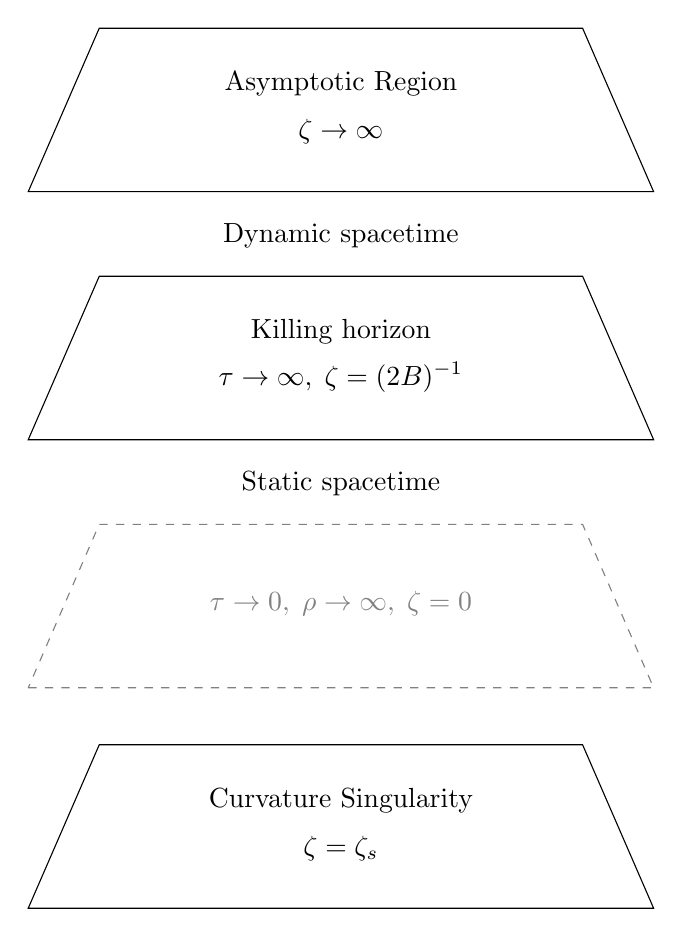
\begin{tikzpicture}[scale=0.7]
\node (I)  at ( 0,-8.5)  {Curvature Singularity};
\node (O)  at ( 0,-4.5)  {};
\node (II)  at (0,0)  {Killing horizon};
\node (III) at (0, 4.5) {Asymptotic Region};
\node (IV) at (0,1.75) {Dynamic spacetime};
\node (V) at (0,-2.75) {Static spacetime};

\path % Singularity Brane
 (I) +(19:-6) coordinate (sbleft)
    +(-19:6) coordinate (sbright)
    +(13:4.5)  coordinate (stright)
    +(-13:-4.5) coordinate (stleft)
    ;
\draw (sbleft) -- node[midway, above, inner sep=6mm] {$\zeta=\zeta_s$} (sbright) -- (stright) -- (stleft) -- (sbleft) -- cycle;

\path % Zero
 (O) +(19:-6) coordinate (sbleft)
    +(-19:6) coordinate (sbright)
    +(13:4.5)  coordinate (stright)
    +(-13:-4.5) coordinate (stleft)
    ;
\draw[gray,dashed] (sbleft) -- node[midway, above, inner sep=9mm] {$\tau \rightarrow 0, \; \rho \rightarrow\infty, \; \zeta=0$} (sbright) -- (stright) -- (stleft) -- (sbleft) -- cycle;

\path % Event Brane
 (II) +(19:-6) coordinate (ebleft)
    +(-19:6) coordinate (ebright)
    +(13:4.5)  coordinate (etright)
    +(-13:-4.5) coordinate (etleft)
    ;

\draw (ebleft) -- node[midway, above, inner sep=6mm] {$\tau \rightarrow \infty, \;  \zeta= (2B)^{-1}$} (ebright) -- (etright) -- (etleft) -- (ebleft) -- cycle;

\path % Asy Brane
 (III) +(19:-6) coordinate (ableft)
    +(-19:6) coordinate (abright)
    +(13:4.5)  coordinate (atright)
    +(-13:-4.5) coordinate (atleft)
    ;

\draw (ableft) -- node[midway, above, inner sep=6mm] {$\zeta \rightarrow \infty$} (abright) -- (atright) -- (atleft) -- (ableft) -- cycle;

\end{tikzpicture}
\caption[Illustration of the spacetime regions of the planar symmetric solutions of the STU model]{Diagram of the spacetime regions. When starting from the 3D solution, a static patch of the spacetime is found, parametrised by $\tau$ for $\zeta \in [0,(2B)^{-1}]$. We can extend this spacetime to a singularity where the Kretschmann invariant becomes infinite. Analytically continuing our parameter through the horizon to $\zeta > (2B)^{-1}$ we obtain a time-dependent geometry.}
\label{fig:branesum}
\end{figure}

\subsection{Finding asymptotic infinity}

We beginning by applying the coordinate change \eq{cchange} to the fields found in \eq{4dsummary} to obtain a line element for our solution in terms of the coordinates $\{t, \rho, x, y\}$, where $\rho \in (2B, \infty)$. 

Beginning with the scalar fields $q_0$, we find that
\begin{equation}
q_0 = \mp \frac{\Ham_0}{W^{1/2}},  \qquad q_A = \pm \frac{\Ham_A}{W^{1/2}},
\end{equation}
where we have defined the harmonic functions
\begin{equation*}
\Ham_a(\rho) := | K_a | \left[\frac{1}{B} \sinh \bigg(\frac{B h_a}{|K_a|}\bigg) + \frac{e^{-\frac{B h_a}{|K_a|}}}{\rho} \right], \quad a=0,\ldots, 3.
\end{equation*}
The warp factor is found to be
\begin{equation*}
  e^{-4\psi} = W(\rho)^{-2},
\end{equation*}
and the Kaluza-Klein scalar transforms as
\begin{equation}
\label{eq:4cmdf2}
    e^\phi = \half (-q_0 q_1 q_2 q_3)^{-\half} = \frac{W(\rho)}{\Ham(\rho)},
\end{equation}
where we have defined a new function which is the product of our harmonic functions:
\begin{equation}
\Ham (\rho) := 2 \sqrt{\Ham_0 \Ham_1 \Ham_2 \Ham_3}    .
\end{equation}
With the expressions for the Kaluza-Klein function and the warp factor, we can write down the line element with our new transverse coordinate
\begin{equation}
\label{eq:4chargerho}
ds^2 = -\frac{W}{\Ham} dt^2 +\frac{\Ham}{W} \frac{d\rho^2}{\rho^4} + \Ham (dx^2 + dy^2).
\end{equation}
We are now interested in looking for where our asymptotic region is. We do this in an identical procedure to how we studied the geodesic motion in Section \ref{sec:emcausal}.

The Lagrangian (energy functional) for transverse geodesics in the metric \eq{4chargerho} is
\begin{equation*}
    \La = -\frac{W}{\Ham} \dot{t}^2 +\frac{\Ham}{W \rho^4} \dot{\rho}^2,
\end{equation*}
where the dot represents differentiation with respect to an affine parameter $\lambda$. Null geodesics satisfy $\La=0$. The constant of motion associated to the timelike Killing vector $k^\mu$ is
\begin{equation*}
    E = - k \cdot u = \frac{W \dot{t}}{\Ham},
\end{equation*}
which can be rearranged to give a differential equation. Upon integration, we obtain an expression for the affine parameter
\begin{equation}
    \dot{\rho} = \pm \sqrt{ \rho^4 E^2}, \qquad \lambda = \pm \int \frac{d\rho}{E \rho^2} .
\end{equation}
This shows that light signals sent from $\rho > 2 B$ reach $\rho = \infty$ in finite affine parameter, whereas $\rho \rightarrow 0$ is reached in infinite affine parameter. Therefore, $\rho \rightarrow 0$ should be interpreted as being at infinite distance and $\rho<2B$ as the exterior region, while $\rho>2B$ is the interior region.

Given this observation, we introduce the new transverse coordinate $\zeta=\rho^{-1}$ so that infinity is now at $\zeta \rightarrow \infty$. It is important to note that in order to reach the limit of $\zeta \rightarrow \infty$ we must cross the Killing horizon located at $\zeta = (2B)^{-1} =: \alpha^{-1}$ into a new, `exterior' region. In the exterior, $\zeta$ is a timelike coordinate and as the line element depends explicitly on $\zeta$, the exterior is non-stationary and as such the solution is interpreted as cosmological.

We also note that for causal information coming from an asymptotic distance, the Killing horizon is a cosmological horizon which is located at a point in time $\zeta = \alpha^{-1}$, and so will be necessarily crossed for all causal geodesics.\footnote{This mandatory crossing can be understood in the same way as all causal geodesics reaching the singularity for the Schwarzschild solution once the horizon has been crossed.} Once the horizon has been crossed, the timelike singularity can be avoided, and geodesics may leave the static patch into a second dynamic patch of spacetime. This statement is justified with calculations later in Section \ref{sec:stucausal}.

Following our coordinate transformation, the metric can be written in the following form
\begin{equation}
\label{eq:3czmet}
ds^2 = -\frac{W(\zeta)}{\Ham(\zeta)} d\eta^2 +\frac{\Ham(\zeta)}{W(\zeta)} d \zeta^2 + \Ham(\zeta) (dx^2 + dy^2).
\end{equation}
Note that we have relabelled the coordinate $t$, which is interpreted as time in the interior, as $\eta$. This is because $t$ becomes a spacelike coordinate in the exterior patch of spacetime, so we instead use the neutral notation $(\eta, \zeta)$ instead of $(t, \rho)$. After the coordinate change, the metric functions are
\begin{equation*}
\begin{aligned}
	W(\zeta) &= 1 - \alpha \zeta, \\
    \Ham_a(\zeta) &= |K_a| \left[\frac{2}{\alpha} \sinh \bigg(\frac{\alpha h_0}{2 |K_a|}\bigg) + e^{-\frac{\alpha h_0}{2 |K_a|}} \zeta \right].
\end{aligned}
\end{equation*}
We will refer to these harmonics in a condensed format by redefining our integration constants such that
\begin{equation*}
     \Ham_a = \left(\beta_a + \gamma_a \zeta \right),
\end{equation*}
where 
\begin{equation*}
	\beta_a = \frac{2 |K_a|}{\alpha} \sinh \bigg(\frac{\alpha h_0}{2 |K_a|}\bigg), \qquad \gamma_a = |K_a| \exp \left({- \frac{2 h_a}{2 |K_a|}} \right).
\end{equation*}
We refer to these linear functions as harmonics from the perspective of the intersecting brane configurations we introduced in Section \ref{sec:intersecting}. We will see in Chapter \ref{ch:brane} that these solutions can be considered as smeared configurations with one transverse dimension, for which a harmonic function is a linear function. 

Finally, we rewrite the gauge fields (\ref{eq:4dgauge}) which will be particularly important when we consider the dimensional uplift of the solution in Chapter \ref{ch:brane} and in our thermodynamic computations in Chapter \ref{ch:triplewick}
\begin{equation}
\label{eq:new4dgauge}
    \begin{aligned}
        F^0_{\zeta \eta} = (\dot{A}^{0})_\eta = -\frac{Q_0}{2 \Ham_0^2}, \qquad \tilde{F}_{A |\zeta \eta} = (\dot{\tilde{A}}_A)_\eta = \frac{P^A}{2\Ham_A^2}.
    \end{aligned}
\end{equation}


\subsection{The dynamic region}

With an appropriate set of coordinates, let us now demonstrate that the metric can be analytically continued to $\zeta > \alpha^{-1}$. We make an intermediate coordinate transformation to advanced Eddington-Finkelstein coordinates
\begin{equation*}
  v = \eta + \zeta_\star, \qquad d\zeta_\star = \frac{\Ham}{W}d\zeta,
\end{equation*}
where we have introduced the tortoise coordinate $\zeta_\star$ such that the metric can be written in the form
\begin{equation*}
 ds^2 =  - \frac{W}{\Ham} dv^2 + 2 d\zeta dv + \Ham (dx^2 + dy^2).
\end{equation*}
This shows that the metric has no singularity at $\zeta = \alpha^{-1}$ and so we can analytically continue the coordinate $\zeta$ to $\zeta > \alpha^{-1}$, and then reverse the coordinate transformation to obtain the metric for the dynamic patch of the spacetime
\begin{equation*}
    ds^2 = - \frac{{W(\zeta)}}{\Ham(\zeta)} d\eta^2 + \frac{\Ham(\zeta)}{{W(\zeta)}} d \zeta^2 + \Ham(\zeta) (dx^2 + dy^2),
\end{equation*}
for $\zeta > \alpha^{-1}$. Note that $W(\zeta)$ is an everywhere negative function within the domain of the dynamic patch of the spacetime. To have a clearer picture of our spacetime, we define a new, always positive function within this domain: $\mathcal{W}(\zeta) := \alpha \zeta - 1$. Using this, we can write down the metric for $\zeta > \alpha^{-1}$ where it is immediately obvious that the coordinate $\zeta$ is timelike. 

The exterior (region II) is the cosmological region where $\zeta$ is timelike and the metric is time-dependent. The interior (region I) is static, for which $\zeta<\alpha^{-1}$ is spacelike and $\eta$ is timelike. As we will see below, the spacetime ends at a timelike singularity located at $\zeta_s$, where $\zeta_s$ is the first zero of $\Ham(\zeta)$. The respective line elements of these two regions are
\begin{equation}
\label{eq:4chargenew}
\begin{aligned}
    ds^2_{I} = - \frac{{W(\zeta)}}{\Ham(\zeta)} d\eta^2 + \frac{\Ham(\zeta)}{{W(\zeta)}} d \zeta^2 + \Ham(\zeta) (dx^2 + dy^2), \\
    ds^2_{II} = - \frac{\Ham(\zeta)}{{\mathcal{W}(\zeta)}} d \zeta^2 + \frac{{\mathcal{W}(\zeta)}}{\Ham(\zeta)} d\eta^2 + \Ham(\zeta) (dx^2 + dy^2). \\
\end{aligned}
\end{equation}

Having found coordinates suitable for describing both regions of our solution, we now start to analyse its properties. Using \eq{gensca} we obtain the following expressions for the physical scalars:
\begin{equation}
\label{eq:stuphysicalscalars}
  z^1 = -i \left( \frac{\Ham_0 \Ham_1 }{\Ham_2 \Ham_3} \right)^{\half}, \quad z^2 = -i \left( \frac{\Ham_0 \Ham_2 }{\Ham_1 \Ham_3} \right)^{\half}, \quad z^3 = -i \left( \frac{\Ham_0 \Ham_3 }{\Ham_1 \Ham_2} \right)^{\half}.
\end{equation}
We can study the asymptotic behaviour of the scalars by taking the limit $\zeta \to \infty$ and we find
 \begin{equation*}
   \Ham_a \simeq | K_a | e^{-\frac{\alpha h_a}{2 |K_a|}} \zeta,
 \end{equation*}
such that the scalars all tend to a constant value, as all $\Ham_a$ depend on $\zeta$ in the same way
\begin{equation*}
	\lim_{\zeta \to \infty} z^A = -i \left( \frac{\gamma_0 \gamma_A^2}{\gamma_1\gamma_2\gamma_3} \right)^{\half}.
\end{equation*}

We can look for the presence of curvature singularities through computing the curvature scalars corresponding to the metric \eq{4chargenew}. Unlike the previous solutions discussed so far, the Ricci scalar is non-zero, and is found to be
\begin{equation}
\label{eq:ricciscalar}
R = \frac{W \left(\Ham^{\prime 2}-2 \Ham \Ham''\right)}{2 \Ham^3},
\end{equation}
where we denote a derivative with respect to $\zeta$ with a prime. The Kretschmann scalar, $K = R^{\mu \nu \rho \sigma}R_{\mu \nu \rho \sigma}$, is given by
\begin{equation}
\label{eq:krescalar}
\begin{aligned}
K &= \frac{3 W^2 \Ham''^2}{\Ham^4} - \frac{2 W \Ham' \Ham''
  \left(4W\Ham'+3 \alpha \Ham\right)}{\Ham^5}
\\ &+ \frac{\Ham'^2 (27
  W^2 \Ham'^2+ 44 \alpha W \Ham \Ham'+20 \alpha ^2
  \Ham^2)}{4\Ham^6}.
\end{aligned}
\end{equation}
We find that both have singular behaviour for the limit of $\Ham(\zeta) \rightarrow 0$. As $\Ham(\zeta)$ is a polynomial of degree four which factorises into four linear polynomials, it will in general have four distinct zeros at $\zeta = \gamma_a \beta_a^{-1}$. The boundary of the spacetime domain is given by the largest of these zeros, or the `first zero of ${\cal H}(\zeta)$', which we denote $\zeta_s$. We remark that $\zeta_s \leq 0$ for all values of the integration constants. Without loss of generality, we assume that the first zero of $\Ham$ will be for $\Ham_0=0$, such that the singularity will occur at
\begin{equation}
\label{eq:4csing}
    \zeta_s = \frac{1 - e^{\frac{\alpha h_0}{Q_0}}}{\alpha} = -\frac{\beta_0}{\gamma_0} \;.
\end{equation}

\subsection{Near horizon geometry}

We can study the near horizon geometry of this solution through making a coordinate transformation
\begin{equation}
\label{eq:nhcc}
    \chi^2 = \zeta - \alpha^{-1}, \qquad d\zeta^2 = 4 \chi^2 d\chi^2 .
\end{equation}
The horizon values of the harmonic functions are finite
\begin{equation*}
  \Ham_a(\alpha^{-1}) = \frac{|K_a|}{\alpha} \exp\left(\frac{\alpha h_0}{2 |K_a|} \right) ,
\end{equation*}
and after the coordinate change, we find
\begin{equation*}
  d\zeta^2 = 4\chi^2 dr^2, \quad \cW = \alpha \chi^{2}, \quad \Ham = \frac{2Z \E}{\alpha^2},
\end{equation*}
where we have defined
\begin{equation*}
  Z := \sqrt{Q_0P^1P^2P^3}, \quad \E := \exp \bigg[\frac{\alpha}{4} \bigg(\frac{h_0}{Q_0} + \frac{h^1}{P^1} + \frac{h^2}{P^2} + \frac{h^3}{P^3} \bigg) \bigg].
\end{equation*}
We now substitute these expressions into our metric to obtain the near-horizon line element
\begin{equation}
\label{eq:nearhorizon}
ds^2 = -\frac{\alpha^3 \chi^2}{2 Z \E} d\eta^2 + \frac{8 Z \E}{\alpha^3} d\chi^2 + \frac{2 Z \E}{\alpha^2} (dx^2 + dy^2).
\end{equation}
With the near horizon approximation, we can study the Hawking temperature (up to a sign) via Wick-rotation of the timelike coordinate $\eta$. First we perform an additional coordinate change
\begin{equation*}
  dR^2 = \left(\frac{8 Z \E}{\alpha^{3}} \right) d\chi^2,
\end{equation*}
to put our line element into the form in which we can compare it with the Rindler line element \cite{Wald:106274}. Performing the Wick-rotation $\eta \rightarrow -i \eta_E$, we ensure that there is no conical singularity by making the identification $\tau \simeq \tau + \beta$, where $\beta$ can be understood as the inverse temperature $\beta = T_H^{-1}$. Following this reasoning, we find that
\begin{equation}
\label{eq:nearhorizontemp}
    2\pi T_H = \pm \frac{\alpha^3}{4 Z \E}.
 \end{equation}
We remember that the sign of the computation is not set through this reasoning, as explained in Section \ref{sec:bhtemperature}. 


\subsection{The extremal limit}
\label{sec:4Dext}

We are interested in the extremal limit of the solution in which the surface gravity of the Killing horizon vanishes. We can compute the surface gravity using the Kodama-Hayward formulation \eq{THK}, where we additionally have knowledge of the sign, and we find
\begin{equation*}
	\kappa = - \half \partial_\zeta \left( \frac{\cW}{\Ham} \right) \bigg|_{\zeta = \alpha^{-1}} = - \half \frac{\alpha}{\Ham(\alpha^{-1})}.
\end{equation*}
This allows us to identify that $\alpha$ should be interpreted as the non-extremality parameter, with the extremal limit: $\alpha \rightarrow 0$. This is consistent with \eq{nearhorizontemp} where we see that $\kappa = 2\pi T_H$. In Section \ref{sec:stucausal}, we will obtain a global depiction of the spacetime and from that, we can set the sign of the temperature from the classification of the trapping horizons.

As this solution is a generalisation of the Nernst solution, we are interested in how the entropy density behaves in the extremal limit. We can read off the entropy density of the solution as the prefactor of the line element for the coordinates $\{x,y\}$ and we see
\begin{equation*}
    S_{BH} = \frac{2 Z \E}{\alpha^2} .
\end{equation*}
Surprisingly, unlike the Nernst solution which had vanishing area density, the entropy density diverges in the extremal limit. 

We can look at the geometry of the solution in the extremal limit, and we find the metric functions are found to be
\begin{equation}
\label{eq:extlim}
    \alpha \rightarrow 0 \quad \Rightarrow \quad \cW(\zeta) \rightarrow -1, \qquad \beta_a \rightarrow h_a \zeta, \qquad     \gamma_a \rightarrow K_a .
\end{equation}
The resulting line element is given by
\begin{equation}
\label{eq:stuextremal}
ds^2 =  - \Ham^{-1}(\zeta) d\eta^2 + \Ham(\zeta) d\zeta^2  + \Ham(\zeta) (dx^2 + dy^2),
\end{equation}
where $\eta, \zeta$ are now everywhere timelike and spacelike respectively, and we understand that the spacetime is static. 

Taking the extremal limit has a dramatic effect on the causal structure of the spacetime, similar to what we have already seen when taking the extremal limit for the planar solutions of Einstein-Maxwell in Section \ref{sec:pemextremal}. As the function $\cW$ becomes constant we find that the location of the horizon is set by $\Ham^{-1} \rightarrow 0$, which occurs when $\zeta \rightarrow \infty$. The horizon location is pushed to $\alpha^{-1} \rightarrow \infty$, and the resulting spacetime is everywhere static with a naked singularity. This change in the causal structure is a general feature of the cosmological, planar symmetric solutions we have studied, which was also seen in the three-charge solutions of \cite{Gutowski:2019iyo}. Further discussion of the relationship between the causal structure and the extremal limit is left for Section \ref{sec:branediscussion}, where we have the additional perspective of these solutions as intersecting brane solutions in higher-dimensional supergravity.


\subsection{The asymptotic limit}

We can probe the geometry of the asymptotic region through taking $\zeta \rightarrow \infty$ and we find that
\begin{equation*}
  \lim_{\zeta \rightarrow \infty} \Ham_a(\zeta) \simeq K_a e^{\frac{\alpha h_a}{2 K_a}}\zeta, \qquad \lim_{\zeta \rightarrow \infty} \Ham(\zeta) \simeq 2 Z \E \zeta^2, \qquad \lim_{\zeta \rightarrow \infty} \cW(\zeta) \simeq \alpha \zeta.
\end{equation*}
We use this to write down the asymptotic metric
\begin{equation}
\label{eq:stuasymptotic}
  ds^2 = - \frac{2 Z \E \zeta}{\alpha} d\zeta^2 + \frac{\alpha}{2 Z \E \zeta} d\eta^2 + 2 Z \E \zeta^2 (d\bar{x}^2 + d\bar{y}^2) ,
\end{equation}
and with a simple change of coordinates to absorb all of the constants, we find the asymptotic metric is in the form
\begin{equation}
\label{eq:asymet}
  ds^2 = - \bar{\zeta} d\bar{\zeta}^2 + \frac{1}{\bar{\zeta}} d\bar{\eta}^2 + \bar{\zeta}^2 (d{x}^2 + d{y}^2).
\end{equation}
We find that the asymptotic geometry is the same as for the planar solutions of Einstein-Maxwell, which we understand as the planar Schwarzschild solution (AIII metric) with the mass $M=\frac{1}{2}$ \cite{Griffiths:2009dfa}. This matching of asymptotic geometries can be understood as in the asymptotic limit, the scalars fall off to a constant value. As we will show in Section \ref{sec:emfromstu}, the solutions of Einstein-Maxwell theory can be recovered from the STU model by imposing all the scalar fields take constant values.

Making the coordinate transformation
\begin{equation*}
  \bar{\eta} = \left(\frac{3}{2}\right)^{\frac{1}{3}} z, \qquad   \bar{\zeta} = \left(\frac{9}{4}\right)^{\frac{1}{3}} \tau^{\frac{2}{3}}, \qquad   (x,y) = \left(\frac{4}{9}\right)^{\frac{1}{3}} (x,y), \qquad
\end{equation*}
we can rewrite the asymptotic metric in the form
\begin{equation*}
  ds^2 = -d\tau^2 + \tau^{2/3} dz^2 + \tau^{4/3} (dx^2 + dy^2),
\end{equation*}
which is the type-D vacuum Kasner solution \cite{Kasner:1921zz}. The Penrose-Carter diagram for the vacuum Kasner type-D solution was given in Figure (\ref{fig:kasnerpc}).


\section{Causal structure of cosmological solutions}
\label{sec:stucausal}
In this section, we use the general framework we built in Section \ref{sec:pemglobal} to draw the Kruskal diagram and the Penrose-Carter diagrams for the planar symmetric solutions of the STU model. We can also carry through the computations to classify the horizons and find that they are \emph{inner horizons}. From the conformal diagram, we realise that our planar symmetric solutions have an intersection with a class of cosmological solutions studied in \cite{Burgess:2002vu, Burgess:2003mk} for the case of generalised Einstein-Maxwell-Dilaton theory and the orientifold constructions in \cite{Cornalba:2003kd}. We then consider the static patch in more detail, studying causal geodesics and the worldlines of stationary massive particles, following the methodology introduced in Section \ref{sec:emconservedcharges}. We find that the singularity repels all timelike geodesics and that stationary massive particles experience negative acceleration with respect to the singularity. Finally, we compute various mass-like parameters associated with the static region of the spacetime. 

\subsection{Kruskal coordinates and the Penrose-Carter diagram}
\label{sec:stukruskalclassification}
Studying the line element for region I \eq{4chargenew}, in which the transverse coordinate $\zeta$ is spacelike, we notice that it is of the form \eq{kruskalgen} when we make the identification
\begin{equation*}
	f(\zeta) = \frac{W(\zeta)}{\Ham(\zeta)} = \frac{1 - \alpha \zeta}{2 \sqrt{(\beta_0 + \gamma_0 \zeta)(\beta_1 + \gamma_1 \zeta)(\beta_2 + \gamma_2 \zeta)(\beta_3 + \gamma_3 \zeta)}}.
\end{equation*} 
As we allowed $f(r)$ to be completely general in our construction of Kruskal-like coordinates of our cosmological solutions in Section \ref{sec:kruskalgen}, we can write down our line element in terms of Kruskal-like coordinates $\{U,V\}$
\begin{equation*}
     ds^2 = - \frac{f(\zeta) e^{-2\kappa \zeta_\star}}{\kappa^2} dV dU + \Ham(\zeta) d\vec{X}^2 \;.
\end{equation*}
From this, we know that the Kruskal diagram for these solutions will be the Figures \ref{fig:coskrus} and \ref{fig:sub2}, which we redraw with explicit labels for each region in Figure \ref{fig:stukruskal}. We can similarly draw the Penrose-Carter diagram for these solutions, which we give in Figure \ref{fig:stuPC}.

We can continue following the generalised discussion in Section \ref{sec:genclassification} to classify the horizons in our spacetime. Region IV is that which we understand as having the conventional time orientation. The horizon separating regions III and IV is a \emph{future inner horizon}, which has a temperature proportional to the surface gravity and so is negative. It is this horizon which we consider when studying the thermodynamics of these solutions in Section \ref{sec:thermostu}. The horizon separating regions IV and II is a \emph{past inner horizon}, which has a temperature with a sign opposite to the surface gravity, and so is positive.

\begin{figure}
  \centering
    \begin{tikzpicture}
    \draw[black!15!white] (0,1) -- (5,4);
    \draw[black!15!white] (0,2) -- (5,3);
    \draw[black!15!white] (0,3) -- (5,2);
    \draw[black!15!white] (0,4) -- (5,1);
    \draw[black!15!white] (1,0) -- (4,5);
    \draw[black!15!white] (2,0) -- (3,5);
    \draw[black!15!white] (3,0) -- (2,5);
    \draw[black!15!white] (4,0) -- (1,5);

    % bottom    
    \draw[black!15!white] (2.5,4.1) parabola (4.65,5);
    \draw[black!15!white] (2.5,4.1) parabola (0.35,5);    
    \draw[black!15!white] (2.5,3.75) parabola (4.8,5);
    \draw[black!15!white] (2.5,3.75) parabola (0.2,5);
    \draw[black!15!white] (2.5,3.4) parabola (4.9,5);
    \draw[black!15!white] (2.5,3.4) parabola (0.1,5);

    % top
    \draw[black!15!white] (2.5,0.9) parabola (4.65,0);
    \draw[black!15!white] (2.5,0.9) parabola (0.35,0);    
    \draw[black!15!white] (2.5,1.25) parabola (4.8,0);
    \draw[black!15!white] (2.5,1.25) parabola (0.2,0);
    \draw[black!15!white] (2.5,1.6) parabola (4.9,0);
    \draw[black!15!white] (2.5,1.6) parabola (0.1,0);
    
    % left
    \begin{scope}[shift={(5,0)}, rotate=90]
    \draw[black!15!white] (2.5,4.1) parabola (4.65,5);
    \draw[black!15!white] (2.5,4.1) parabola (0.35,5);    
    \draw[black!15!white] (2.5,3.75) parabola (4.8,5);
    \draw[black!15!white] (2.5,3.75) parabola (0.2,5);
    \draw[black!15!white] (2.5,3.4) parabola (4.9,5);
    \draw[black!15!white] (2.5,3.4) parabola (0.1,5);
    \end{scope}
    
    % right
    \begin{scope}[shift={(0,5)}, rotate=-90]
    \draw[black!15!white] (2.5,4.1) parabola (4.65,5);
    \draw[black!15!white] (2.5,4.1) parabola (0.35,5);    
    \draw[black!15!white] (2.5,3.75) parabola (4.8,5);
    \draw[black!15!white] (2.5,3.75) parabola (0.2,5);
    \draw[black!15!white] (2.5,3.4) parabola (4.9,5);
    \draw[black!15!white] (2.5,3.4) parabola (0.1,5);
    \end{scope}
    
    \draw[thick, ->] (0,0) -- node[at end, above=0.3cm]{$V$} (5,5);
    \draw[thick, ->] (5,0) -- node[at end, above=0.3cm]{$U$} (0,5);
    
    \draw[thick, red!90!white, ->-] (0,2.5) -- (2.5,5);
    \draw[thick, blue!90!white, ->-] (2.5,0) -- (0,2.5);
    
    \draw[thick, white] (0,0.5) edge  (0,4.5)
         edge[bend right,fill=white, draw=black, thin] node[rotate=90, midway,above, black,  font=\fontsize{10}{0}] {$\zeta=0$} (0,4.5);
         
    \draw[thick, white] (5,0.5) edge  (5,4.5)
         edge[bend left,fill=white, draw=black, thin] node[rotate=90, midway,below, black,  font=\fontsize{10}{0}] {$\zeta=0$} (5,4.5);
         
    \draw[thick, white] (0.5,0) edge  (4.5,0)
         edge[bend left,fill=white, draw=black, thin] node[midway,below=0.25cm, black,  font=\fontsize{10}{0}] {$\zeta=\infty$} (4.5,0);
    
    \draw[thick, white] (0.5,5) edge  (4.5,5)
         edge[bend right,fill=white, draw=black, thin] node[midway,above=0.25cm, black,  font=\fontsize{10}{0}] {$\zeta=\infty$} (4.5,5);
    
    \node (a) at (3.3,2.5) {I};
    \node (a) at (1.6,2.5) {IV};
    \node (a) at (2.5,3.5) {II};
    \node (a) at (2.5,1.6) {III};
    \end{tikzpicture}
\caption[Kruskal diagram for the planar symmetric solutions of the STU model]{Kruskal diagram for the planar symmetric solutions of the STU model, which we can draw from the qualitative similarity of this solution to the general discussion given in Section \ref{sec:pemglobal}. As before, ingoing (outgoing), transverse null geodesics are drawn in blue (red).}
\label{fig:stukruskal}
\end{figure}

\begin{figure}[h!]
\centering
\begin{tikzpicture}
\node[above] (0) at (0.13,12) {$i^+$};
\node[below] (1) at (0.13,-4) {$i^-$};
\node (I) at (0,8) {II};
\node (II) at (0,0) {III};
\node (III) at (-2.5,4) {IV};
\node (IV) at (2.5,4) {I};
\path % Four corners of left diamond
 (I) +(90:4) coordinate[label=90:] (IItop)
 +(-90:4) coordinate(IIbot)
 +(0:4) coordinate[label=360:] (IIright)
 +(180:4) coordinate[label=180:] (IIleft)
 ;
\draw (IIleft) --
 node[midway, below, sloped] {$\zeta=\infty, \eta = - \infty$}
 (IItop) --
 node[midway, below, sloped] {$\zeta=\infty, \eta = \infty$}
 (IIright)
     node[midway, above, sloped] {$\mathcal{J}^+$}
           --
 node[midway, above, sloped] {$\zeta = \alpha^{-1}$}
 (IIbot) --
 node[midway, above, sloped] {$\zeta = \alpha^{-1}$}
 (IIleft) -- cycle;


\path % Four conners of the right diamond (no labels this time)
 (II) +(90:4) coordinate (Itop)
 +(-90:4) coordinate (Ibot)
 +(180:4) coordinate (Ileft)
 +(0:4) coordinate (Iright)
 ;
% No text this time in the next diagram
\draw (Ileft) --
 node[midway, below, sloped] {$\zeta = \alpha^{-1}$}
 (Itop) --
 node[midway, below, sloped] {$\zeta = \alpha^{-1}$}
 (Iright) --
 node[midway, above, sloped] {$\zeta=\infty, \eta = - \infty$}
 (Ibot) --
 node[midway, above, sloped] {$\zeta=\infty, \eta = \infty$}
 node[midway, below, sloped] {$\mathcal{J}^-$}
 (Ileft) -- cycle;

%Squiggly lines
\draw[decorate,decoration=snake,draw=black] (Ileft) -- (IIleft)
 node[midway, above, sloped] {$\zeta_s$};

\draw[decorate,decoration=snake, draw=black] (Iright) -- (IIright)
 node[midway, below, sloped] {$\zeta_s$};

\draw[blue,dashed,bend right=25, thick] (Ileft) to (Iright);
\draw[blue,dashed,bend right=-25, thick] (Ileft) to (Iright);
\draw[blue,dashed,bend right=25, thick] (IIleft) to (IIright);
\draw[blue,dashed,bend right=-25, thick] (IIleft) to (IIright);
\draw[blue,dashed,bend right=25, thick] (Ileft) to (IIleft);
\draw[blue,dashed,bend right=-25, thick] (Iright) to (IIright);
\draw[->-,orange,bend right=-20, thick] (1) to (0);


\end{tikzpicture}
\caption[Penrose-Carter diagram for the planar cosmological solutions of the STU model]{Penrose-Carter diagram for the planar cosmological solutions. Starting at $\zeta \rightarrow \infty$, we have a cosmological spacetime (III) with a future inner horizon located at a finite point in time; any observer must necessarily fall through the horizon. Passing through the horizon, the spacetime is static (IV) with an avoidable (repulsive) naked singularity located at a point in space. Massive particles at rest experience negative acceleration and will leave the static region through a past inner horizon, into a second dynamic spacetime (I). An example of a complete timelike geodesic is given in orange, spacelike hypersurfaces of constant time are given in blue.}
\label{fig:stuPC}
\end{figure}

\subsection{Geodesic motion}

Following the computations performed in Section \ref{sec:emgeodesics}, we can study the timelike and null geodesics of the solution through considering the Lagrangian
\begin{equation}
    s = \La = - \frac{W(\zeta)}{\Ham(\zeta)} \dot{\eta}^2 + \frac{\Ham(\zeta)}{W(\zeta)} \dot{\zeta}^2 + \Ham (\dot{x}^2 + \dot{y}^2),
\end{equation}
where $s=0,-1$ for null and timelike geodesics respectively (we will not consider spacelike geodesics for which $s = 1$). We calculate the constants of motion from the isometries as
\begin{equation*}
    E = \frac{W}{\Ham} \dot{\eta}, \qquad a = \Ham \dot{x}, \qquad b = \Ham \dot{y} ,
\end{equation*}
allowing us to rewrite the Lagrangian as
\begin{equation}
    s\frac{W}{\Ham} = -E^2 + \dot{\zeta}^2 + (a^2 + b^2)\frac{W}{\Ham^2}.
\end{equation}
Collecting the terms together and separating out an effective potential, we can write the differential equation into the suggestive form 
\begin{equation}
    \dot{\zeta}^2 = E^2 - V(\zeta), \qquad V(\zeta) = \frac{W}{\Ham} \left(-s + \frac{a^2 + b^2}{\Ham} \right),
\end{equation}
which can be interpreted as the equation of motion for a particle with mass $m=2$. The domain of validity for the equation of motion is restricted by the inequality
\begin{equation*}
    V(\zeta) \leq E^2.
\end{equation*}
The point at which $V(\zeta_0)=E$ is interpreted as the classical turning point of the particle's trajectory. Studying the potential $V(\zeta)$ for the domain in which $\zeta$ is spacelike, we can look at the motion of causal information along geodesics.

\begin{figure}[h!]
\centering
\begin{tikzpicture}[scale=1.5]
 \draw[->] (-1,0.6) -- (5,0.6) node[right] {$\zeta$};
 \draw[->] (0,-2) -- (0,3) node[above] {$V(\zeta)$};
 \draw[dashed,red] (-.6,-2) -- (-.6,3);
 \draw[black] (1.6,0.5) -- (1.6,0.7);
     \draw[domain=-.55:4.8,smooth,variable=\x,blue,thick] plot({\x},{(30 -\x)/((3*\x+5)*(3*\x+5)) + 0.3});
     \node[left] (one) at (-0.5,0.3) {$-\frac{\beta_0}{\gamma_0}$};
     \node[left] (one) at (2,0.35) {$\alpha^{-1}$};
\end{tikzpicture}
\caption[The effective potential for the motion of geodesics in the planar symmetric solutions of the STU model]{Behaviour of the effective potential as a function of $\zeta$ for the set of causal geodesics excluding null transverse geodesics, for which $V(\zeta) = 0$.}
\label{fig:3pot}
\end{figure}

In Figure \ref{fig:3pot} we plot $V(\zeta)$ and see that for region I, in which $\zeta < \alpha^{-1}$, the potential is everywhere positive and therefore considered repulsive. When decreasing $\zeta$ from $\alpha^{-1}$ towards $\zeta_s$, we see that the potential monotonically increases until it diverges in the limit of the singularity. As such, we are guaranteed a unique solution for $V(\zeta_0) = E^2$, and hence the existence of a classical turning point. There is one exception to this, the case when $s = a = b = 0$, specific to the motion along transverse null geodesics, where the potential is everywhere zero. In this case, there is no turning point and the transverse, null geodesic reaches $\zeta = \zeta_s$ in finite affine parameter:
\begin{equation*}
	\lambda = \pm \int \frac{1}{E^2} d\zeta = \pm \frac{1}{E^2} \left( \zeta_0 - \zeta_s \right),
\end{equation*}
evaluated from some initial point $\zeta_0 > \zeta_s$. We realise that our spacetime is not geodesically complete.
    
We can understand this repulsive potential from another perspective through looking at the proper acceleration for a massive particle at rest at some point in region (I/IV) of the spacetime. We consider a massive particle following the orbit of the stationary Killing vector field $k^\mu = \partial_\eta$. The norm of the Killing vector field is given by
\begin{equation*}
	k^2 = - \frac{W}{\Ham},
\end{equation*}
and the only non-zero component  of the proper acceleration \eq{properacccomp} is found to be
\begin{equation}
A^\zeta = - \frac{\alpha \Ham + W \partial_\zeta \Ham}{\Ham^2}.
\end{equation}
As the functions $W$, $\Ham$ and $\partial_\zeta \Ham$ are everywhere positive in the static region of spacetime, we see $A^\zeta < 0$, and that a particle at rest always experiences a force repelling it from the singularity. 
   
We can understand the behaviour as qualitatively identical the planar Einstein-Maxwell solution discussed in Section \ref{sec:emcausal}. The metric functions $\Ham(\zeta)$ and $W(\zeta)$ produce a line element with a more `complicated' form, but from the point of view of the global structure, we see no difference. This leads us to the same conclusion for the movement of geodesics. For non-zero potentials, a particle will arrive from $\mathcal{J}^-$ and necessarily fall through the horizon at $\zeta = \alpha^{-1}$, which is located at a point in time. The particle will then continue towards the singularity to a minimum distance $\zeta_0$, which is the classical turning point. At this point, the particle will then be reflected by the singularity and continue off through the Killing horizon into a second dynamic spacetime towards $\mathcal{J}^+$. The only causal geodesics which do not follow these trajectories are those for which $V(\zeta)=0$. These are precisely the transverse null geodesics which fall through the horizon from $\mathcal{J}^-$ and straight into the singularity. In Figure \ref{fig:stuPC}, an example of a geodesically complete timelike curve is drawn in orange.

\subsection{Mass}
\label{sec:stumass}
We now turn our attention into looking at the mass-like quantities we can compute within the static region of the spacetime. Computation of the conserved electric and magnetic charges of this solution is delayed until Section \ref{sec:thermostu}. When verifying the first law, we will find it helpful first to dualise our gauge fields, so the solution is purely electric. The computation of conserved charges is better suited within the context of the Euclidean action formalism, which can be done whilst also performing the dualisation, where we compute an exact form for the gauge couplings as functions of $\zeta$. For reference, the charges are given in equations \eq{stuq}, \eq{stup}.

As in Section \ref{sec:emconservedcharges}, we will consider both the Komar formalism, as well as quasi-local Brown-York formalism. For both methods, the mass quantity is extracted from the energy by taking an asymptotic limit. However, both of these formalisms assume the spacetime region to be stationary, and as our static region is finite, taking the asymptotic limit brings us into a region in which our initial assumptions no longer hold. As a result, we cannot interpret the asymptotic evaluation of the energy quantities as mass-like. To remedy this, we do not take the limit and instead find the Komar energy, and quasi-local energy as position-dependent quantities. This methodology is inspired by the computations performed in \cite{Burgess:2002vu, Burgess:2003mk}, and mirrors the work already discussed in Section \ref{sec:emcausal}. 

\subsubsection*{Komar mass}

The Komar energy \eq{komarenergy}, repeated here,
\begin{equation*}
	E_{K} = - \frac{1}{8\pi} \int_{\Real^2} \star dk ,
\end{equation*}
is computed from our timelike Killing vector $k$. We again mention our inability to properly normalise this quantity. In spherically symmetric solutions, the Killing vector is normalised such that $k^2 = -1$ in the asymptotic limit, but for these planar symmetric solutions, $k^2 \rightarrow 0$ in the limit of $\zeta \rightarrow \infty$. Because of this, we leave $k^2$ unnormalised and study the Komar energy as a position dependent quantity in spacelike $\zeta$.

For the Killing vector: $k^\mu = (\partial_\eta,0,0,0)$ and taking the Hodge dual, with orientation set by $\epsilon_{\eta \zeta x y} = 1$, we find
\begin{equation*}
    (\star dk)_{\eta \zeta} = -\Ham \partial_\zeta \left( \frac{W}{\Ham} \right) .
\end{equation*}
The Komar integral is evaluated to
\begin{equation*}
        E_K = -\frac{1}{8\pi} \int_{\Real^2} \left(\alpha + \frac{W}{\Ham} \partial_{\zeta} \Ham \right) .
\end{equation*}
Due to the planar symmetry of our solution, this value is divergent when integrating over the plane, so we instead work with the energy density. The resulting position dependent energy density is
\begin{equation}
    E_K = - \left( \frac{\alpha}{8 \pi} + \frac{\partial_\zeta \Ham}{8 \pi} \frac{W}{\Ham} \right).
\end{equation}
Within the domain of the static region $\Ham, W, \partial \Ham > 0$, so as $\alpha$ is positive, the Komar energy will be everywhere negative, regardless of the overall normalisation of $k^2$. We can play the same game we did in Section \ref{sec:emconservedcharges} and take the asymptotic limit, despite having no physical motivation. Doing this, we find that it is finite
\begin{equation*}
	M_{K} = \frac{\alpha}{8 \pi},
\end{equation*} 
and that like the planar solutions to Einstein-Maxwell, this asymptotic energy contribution depends only on the non-extremality parameter. 

\subsubsection*{Brown-York mass}

Now let us compute the Brown-York energy, using the integral \eq{BYmass}, repeated here
\begin{equation}
E_{BY} = -\frac{1}{8 \pi} \int_{\Real^2} \sqrt{\sigma} (\mathtt{k} - \mathtt{k}_0),
\end{equation}
where $\mathtt{k}$ is the extrinsic curvature of the codimension-two manifold embedded into our spacetime. Comparing our metric \eq{4chargenew} with the ADM decomposition \eq{ADM} we identify
\begin{equation*}
N^2 = \frac{W}{\Ham}, \quad V^i = 0, \quad \sigma_{xx} = \sigma_{yy} = \Ham.
\end{equation*}
The quasi-local energy is then calculated using these quantities together with the trace of the extrinsic curvature
\begin{equation}
\mathtt{k} = \frac{1}{\Ham} \sqrt{\frac{W}{\Ham}}\partial_{\zeta} \Ham.
\end{equation}

As with the Komar energy, we have no natural way to normalise this energy, albeit for a different reason. As discussed in Section \ref{sec:emconservedcharges}, the normalisation for the Brown-York energy comes from picking a suitable background, from which we compute $\mathtt{k}_0$. The most conventional choice, when available, is to use the maximally symmetric space located in the asymptotic limit. In Section \ref{sec:brownyorkmass}, we saw this with the Reissner-Nordstr\"om solution, where the divergent energy became finite after we removed the `infinite energy contribution' from the Minkowski background. Another choice for solutions with electromagnetic charges is to use the extremal solution as the background geometry. The issue with normalisation here is two-fold. Firstly, these normalisations come into play when we choose to set the boundary in the asymptotic region. For these cosmological solutions, this limit brings us into a non-stationary region of the spacetime, thus breaking an initial assumption of the formalism. The second is that even if we accept the limit as a valid concept, neither the background contributions derived from the asymptotic region \eq{stuasymptotic}, or the extremal line element \eq{stuextremal} cancel the divergence as $\zeta \to \infty$ which grows as $\Op(\sqrt{\zeta})$. As a result, we study the energy without normalisation, setting $\mathtt{k}_0 = 0$.

Inserting the various pieces into the integral, we find the Brown-York energy
\begin{equation}
\begin{aligned}
E_{BY} &= -\frac{1}{8 \pi} \int d^2 x \sqrt{\sigma} \mathtt{k}, \\
        &= - \frac{1}{8 \pi} \int d^2x \sqrt{\frac{W}{\Ham}}\partial_{\zeta} \Ham.
\end{aligned}
\end{equation}
From the point of view of energy density, we calculate
\begin{equation}
E_{BY} = - \frac{\partial_{\zeta} \Ham}{8 \pi} \sqrt{\frac{W}{\Ham}}.
\end{equation}
This is negative-definite in the static domain due to identical reasoning as for the Komar calculation.

If instead of following the Brown-York mass, we follow the Katz-Lynden-Bell-Israel formalism and include the lapse function, we find that the energy contribution is given by
\begin{equation*}
E_{KLBI} = -\frac{1}{8 \pi} \int_{\Real^2} \sqrt{\sigma} N (\mathtt{k} - \mathtt{k}_0),
\end{equation*}
which for our current solution, gives the energy density
\begin{equation}
E_{KLBI} = - \frac{\partial_{\zeta} \Ham}{8 \pi} \frac{W}{\Ham} .
\end{equation}
Comparing this with the Brown-York energy, we see introducing the lapse function has no effect on the sign within the static region. However, the Katz-Lynden-Bell-Israel energy does have an interesting property of being finite if we take the (inappropriate) asymptotic limit. Taking the limit of the boundary to $r \rightarrow \infty$, we find that the energy is real and finite
\begin{equation*}
	M_{KLBI} = \lim_{r \rightarrow \infty} E_{KLBI} = \frac{\alpha}{4 \pi}.
\end{equation*}
and like the Komar mass, depends only on the non-extremality parameter. We will revisit the mass when we understand it as the internal energy of the solution from a thermodynamic perspective. In Section \ref{sec:stufirstlaw}, the mass is computed and we find
\begin{equation*}
	M = \frac{1}{16\pi} \frac{\alpha}{\sqrt{\gamma_0 \gamma_1 \gamma_2 \gamma_3}}.
\end{equation*}
Note that unlike the planar solutions of Einstein-Maxwell, there is a difference between this mass and the Komar mass computed above. This difference comes from a change of coordinates we make in Section \ref{sec:studynamicthermo}, where we impose that the metric over the two-plane falls off as 
\begin{equation*}
	ds^2_2 = \zeta^2 (d\bar{x}^2 + d\bar{y}^2),
\end{equation*}
when we take the limit $\zeta \to \infty$. We find that these planar coordinates are related by 
\begin{equation*}
	(x, y) \mapsto 2 \sqrt{\gamma_0 \gamma_1 \gamma_2 \gamma_3} \; (\bar{x}, \bar{y}),
\end{equation*}
and if we make this coordinate change on the line element for region I in \eq{4chargenew} and recompute the Komar energy, we find
\begin{equation*}
        E_K = -\frac{1}{16\pi} \frac{1}{\sqrt{\gamma_0 \gamma_1 \gamma_2 \gamma_3}} \int_{\Real^2} \left(\alpha + \frac{W}{\Ham} \partial_{\zeta} \Ham \right) .
\end{equation*}
Again evaluating for $\zeta \to \infty$ we obtain
\begin{equation}
\label{eq:rescaledstumass}
	M_K = M = \frac{1}{16\pi} \frac{\alpha}{\sqrt{\gamma_0 \gamma_1 \gamma_2 \gamma_3}}.
\end{equation}
Showing that these two quantities can be made to be equal through coordinate changes says less about the validity of the solution and more about our inability to know the correct normalisation without some additional information. We see that when considering these position dependent quantities in the static region, the best we can hope for is an understanding of the overall sign of the energy. In Section \ref{sec:thermostu}, we are able to find an overall normalisation for the Euclidean action by imposing that the thermodynamic derivation for the conserved charges matches Gauss' law. It is this new `boundary condition', which gives us a foothold to go from, which then leads to the verification for the first law of thermodynamics.


\section{Recovering the planar solution of Einstein-Maxwell theory}
\label{sec:emfromstu}
If we take the limit of setting the physical scalars of the theory to be constant, the geometry of the four-charge solution becomes that of the vacuum solution to the Einstein-Maxwell equations with planar symmetry, studied in Chapter \ref{ch:planarem}. This is expected as the Reissner-Nordstr\"om solution is the resulting geometry for the spherically symmetric solution to the STU model with constant physical scalars. This matching of solutions can be understood as the non-extremal generalisation of the double-extremal limit \cite{Ferrara:1997tw}.

To reiterate, the physical scalars are given by
\begin{equation*}
    z^A = -i \Ham_A \bigg(\frac{\Ham_0}{\Ham_1 \Ham_2 \Ham_3} \bigg)^{\frac{1}{2}},
\end{equation*}
and we see that they are everywhere constant under the restriction that all the harmonics are equal: $\Ham_0 = \Ham_1 = \Ham_2 = \Ham_3$. This is achieved by fine-tuning the integration constants such that $Q_0 = P^1 = P^2 = P^3 = K$ and $h_0 = h^1 = h^2 = h^3 = h$.

Understanding that the scalar fields are constant after imposing this matching condition on the integration constants, we can look at how the Lagrangian \eqref{eq:4dlag} changes in this limit. As the scalar fields are constant, the kinetic term for the scalar field vanishes. The gauge coupling $\I_{IJ}$ depends only on the scalar fields, and so is itself a constant. The four gauge fields $F^I$ are all equal and so we can reinterpret the contribution from the $n_V + 1$ gauge fields as a single gauge field contribution. All that remains of \eqref{eq:4dlag} is the Ricci scalar and a single Abelian gauge field and so by a suitable rescaling of $F$, the action can be brought into the form of the Einstein-Maxwell Lagrangian \eqref{eq:EMaction}.

This transition from the STU model to the Einstein-Maxwell theory is also mirrored in our geometry. When we take the above limit for our integration constants, we recover the line element for the solution of Einstein-Maxwell theory with planar symmetry \eq{planareinsteinmaxwell}. The metric for the static patch of the spacetime, repeated here
\begin{equation}
\label{eq:genmet}
    ds^2 = - \frac{W(\zeta)}{\Ham(\zeta)} d\eta^2 + \frac{\Ham(\zeta)}{W(\zeta)} d\zeta^2  + \Ham(\zeta) (dx^2 + dy^2),
\end{equation}
changes at the level of these functions, which are now given by
\begin{equation*}
 W(\zeta) = 1 - \alpha \zeta, \qquad \Ham(\zeta) = 2(\beta + \gamma \zeta)^2,
\end{equation*}
with our integration constants simplified as
\begin{equation*}
    \alpha = 2B, \quad \beta =\frac{2 K}{\alpha} \sinh\left(\frac{\alpha h}{2 K}\right), \quad \gamma = K \exp\left(-\frac{\alpha h}{2 K}\right), \qquad \alpha,\beta,\gamma \in (0, \infty).
\end{equation*}
The metric written in terms of these new constants for $\zeta < \alpha^{-1}$ is given by
\begin{equation}
\label{eq:global}
  ds^2 = - \frac{1 - \alpha \zeta }{2(\beta + \gamma \zeta)^2} d\eta^2 + \frac{2(\beta + \gamma \zeta)^2}{(1 - \alpha \zeta )} d\zeta^2  + 2(\beta + \gamma \zeta)^2(dx^2 + dy^2).
\end{equation}

We now show that a suitable change in coordinates maps this line element into our solution \eq{planareinsteinmaxwell}, derived in Chapter \ref{ch:planarem} which we repeat here for comparison
\begin{equation*}
  ds^2 =  - f(r) dt^2 + \frac{dr^2}{f(r)}  + r^2(dx^2 + dy^2), \qquad   f(r) = -\frac{2M}{r} + \frac{Q^2}{r^2}.
\end{equation*}

The equivalence of our solution \eq{genmet} and \eq{planareinsteinmaxwell} is found after making the following coordinate transformations
\begin{equation*}
    2(\beta + \gamma \zeta)^2 = \tilde{r}^2 \; \Rightarrow \; \tilde{r} = \sqrt{2} (\beta + \gamma \zeta), \qquad \zeta = \frac{1}{\gamma} \left(\frac{\tilde{r}}{\sqrt{2}} -\beta \right), \qquad d\zeta = \frac{d\tilde{r}}{\sqrt{2} \gamma},
\end{equation*}
we can then rewrite parts of the line element as
\begin{equation*}
\begin{aligned}
         \frac{1 - \alpha \zeta }{2(\beta + \gamma \zeta)^2} d\eta^2 &= \left(-\frac{\alpha}{\sqrt{2} \gamma \tilde{r}} + \frac{\alpha \beta + \gamma}{\gamma \tilde{r}^2} \right) d\eta^2, \\
         \frac{2(\beta + \gamma \zeta)^2}{(\alpha \zeta - 1)} d\zeta^2 &=  \left(-\frac{\alpha}{\sqrt{2} \gamma \tilde{r}} + \frac{\alpha \beta + \gamma}{\gamma \tilde{r}^2} \right)^{-1} \frac{d\tilde{r}^2}{2 \gamma^2}.
\end{aligned}
\end{equation*}
To ensure that the functions preceding the $d\eta^2$ and $d\tilde{r}^2$ are each other's multiplicative inverse we rescale $\tilde{r}$ such that
\begin{equation*}
    r = \frac{\tilde{r}}{\sqrt{2} \gamma}, \qquad dr = \frac{d\tilde{r}}{\sqrt{2} \gamma}, \qquad \tilde{r} = \gamma \sqrt{2} r.
\end{equation*}
This allows us to write down the metric in the form
\begin{equation*}
  ds^2 = - f(r) d\eta^2 + \frac{dr^2}{f(r)} + 2 \gamma^2 t^2(dx^2 + dy^2),
\end{equation*}
where we have defined the function
\begin{equation*}
    f(r) := - \frac{\alpha}{2 \gamma^2} \frac{1}{r} + \frac{\alpha \beta + \gamma}{2 \gamma^3} \frac{1}{r^2}.
\end{equation*}
Finally we rescale the $x$ and $y$ coordinates to re-absorb the $2 \gamma^2$ factor and rename $\eta$ to $t$ to arrive at the metric
\begin{equation}
  ds^2 = - f(r) dt^2 + \frac{dr^2}{f(r)} + r^2(dx^2 + dy^2).
\end{equation}
Looking at the function $f(r)$ and comparing this to \eq{planareinsteinmaxwell} we can relate the integration constants from our solution to the `mass' and electric charge of the solution.
\begin{equation}
\label{eq:mapintconstants}
    M = \frac{\alpha}{4 \gamma^2}, \qquad Q^2 = \frac{\alpha \beta + \gamma }{2\gamma^3}.
\end{equation}

Thinking back to the asymptotic limit of the Komar energy for planar solution Einstein-Maxwell theory \eq{pemkomar} and for the STU model after rescaling \eq{rescaledstumass}
\begin{equation*}
	M_{EM} = \frac{M}{4 \pi}, \qquad M_{STU} = \frac{1}{16\pi} \frac{\alpha}{\sqrt{\gamma_0 \gamma_1 \gamma_2 \gamma_3}} = \frac{\alpha}{16\pi \gamma^2},
\end{equation*}
we see that by making the identification \eq{mapintconstants}, these mass-like parameters match exactly. Furthermore, these masses are precisely the masses we derive from a thermodynamic perspective in Chapter \ref{ch:triplewick}.


\section{Summary}

In this chapter we have derived and studied planar symmetric solutions of $\N = 2$ supergravity in four dimensions. In particular, we have found non-extremal, cosmological solutions of the STU model containing a Killing horizon, which are asymptotic to the type-D Kasner spacetimes. As explained throughout this chapter, the causal structure of this solution matches that of the planar solutions of Einstein-Maxwell theory, so we will not repeat ourselves here. We concluded the chapter by showing that in the limit of ensuring that all the physical scalars $z^A$ are constant, the planar symmetric solution of the STU model becomes that of the Einstein-Maxwell theory. This behaviour is expected as this has already been seen for the case when the solutions are spherically symmetric  \cite{Ferrara:1997tw}.

The initial motivation for this work was to generalise the Nernst solutions discussed in \cite{Dempster:2015}. As a result, we are biased towards considering the thermodynamics of this solution and its behaviour in the extremal limit. The defining property of the Nernst branes is that the area density of the horizon vanishes in the extremal limit, which has a formal analogy with the strict third law of thermodynamics. However, when taking the extremal limit for these solutions, we instead find that the area density diverges and the resulting spacetime is static with a naked singularity. To better understand this extremal behaviour, we study these solutions in higher dimensions. This is the topic of Chapter \ref{ch:brane}.

Furthermore, we are interested in whether these solutions have Killing horizons which obey the first law of black hole mechanics. When attempting to find a mass-like parameter, we concluded that there was no natural method to set the overall normalisation of the mass and our value was inherently position dependent. As the first law is a differential relationship, we are unable to verify the first law without additional structure. In Chapter \ref{ch:triplewick}, we introduce a novel formulation of the Euclidean action formalism, which when considered together with using Gauss' law as an effective boundary condition allows for the verification for the first law.

As further discussion of this solution is dependent on the results of other chapters of this thesis, we prolong a discussion of the planar solutions of the STU model until further results have been presented.

